\chapter{Quantum Circuits}

The allowed operations on (pure) quantum states are those that map normalized states to normalized states, namely unitary operators $U$, satisfying $UU^{\dagger}=U^{\dagger}U=I$. To have a sensible notion of efficient computation, we require that the unitary operators appearing in a quantum computation are realized by quantum circuits. We are given a set of gates, each of which acts on one or two qubits at a time (meaning that it is a tensor product of one or two qubit operator with the identity operator on the remaining qubits). A quantum computation begins in the $\ket{0}$ state, applies a sequence of one and two qubit gates chosen from the set of allowed gates, and finally reports an outcome obtained by measuring in the computational basis.

A quantum circuit (also called quantum network or quantum gate array) generalizes the idea of classical circuit families, replacing the AND, OR, and NOT gates by elementary quantum gates. A quantum gate is a unitary transformation on a small (usually 1,2, or 3) number of qubits). We saw a number of examples already: the bitflip gate X, the phaseflip gate Z, the Hadamard gate H. The main 2-qubit gate we have seen is the controlled-NOT (CNOT) gate. Adding another control qubit, we get the 3-qubit Toffoli gate, also called controlled-controlled-not (CCNOT) gate. This negates the third bit of its input if both of the first two bits are 1. The Toffoli gate is important because it is complete for classical reversible computation: any classical computation can be implemented by a circuit of Toffoli gates. This is easy to see: using auxiliary wires with fixed values, toffoli can implement AND (fix the 3rd ingoing wire to 0) and NOT (fix the 1 st and 2nd ingoing wire to 1). It is known that And and NOT-gates together sufficient to implement any classical Boolean circuit, so if we can apply (or simulate) Toffoli gates, we can implement any classical computation in a reversible manner.

Mathematically, such elementary quantum gates can be composed into bigger unitary operations by taking tensor products (if gates are applied in parallel to different parts of the register), and ordinary matrix products (if gates are applied sequentially). We have already seen a simple example of such a circuit of elementary gates in the previous chapter, namely to implement teleportation.

As in the classical case, a quantum circuit is a finite directed acyclic graph of input nodes, gates, and output node. There are n nodes that contain the input (as classical bits); in addition we may have some more input nodes that are initially $\ket{0}$ (``workspace"). The internal nodes of the quantum circuit are quantum gates that each operate on at most two or three qubits of the state. The gates in the circuit transform the initial state vector into a final state, which will generally be a superposition. We measure some or all qubits of this final state in the computational basis in order to (probabilistically) obtain a classical output to the algorithm. We can think of the measurement of one qubit in the computational basis as one special type of gate. We may assume without much loss of generality that such measurements only happen at the very end of the circuit. 

What about the more general kinds of measurements? If we want to apply such a measurement in the circuit model, we will have to implement it using a circuit of elementary gates followed by a measurement in the computational basis. For example, suppose projectors $P_0$ and $P_1$ both have rank $2^n/2$. Then there exists a unitary $U$ that maps an n-qubit state $\ket{\phi}$ to a state whose first qubit is $\ket{1}$ whenever $P_1\ket{\psi}=\ket{\psi}$. We can now implement the projective measurement by first applying a circuit that implements $U$, and then measuring (in the computational basis) the first qubit of the resulting state. The minimal-size circuit to implement $U$ could be very large (i.e. ,expensive) if the projective measurement is complicated, but that is how it should be.

To draw quantum circuits, the convention is to let time progress from left to right: we start with the initial state on the left. Each qubit is pictured as a horizontal wire, and the circuit prescribes which gates are to be applied to which wires. Single-qubit gates like X and H just act on one wire, while multi-qubit gates such as the CNOT act on multiple wires simultaneously. When one qubit "controls" the application of a gate to another qubit, then the controlling wires is drawn with a dot linked vertically to the gate that is applied to the target qubit. This happens for instance with the CNOT, where the applied single-qubit gate is X, usually drawn as $\oplus$ in a circuit picture (similarly, the Toffoli gate is drawn in a circuit with a dot on the two control wire and an $\oplus$ on the target wires).

Note that if we have a circuit for unitary $U$, it is very easy to find a circuit for the inverse $U^{-1}$ with the same complexity: just reverse the order of the gates, and take the inverse of each gate. For example, if $U=U_1U_2U_3$, then $U^{-1}=U_3^{-1} U_2^{-1}U_1^{-1}$.


A more efficient way to describe sequences of quantum operations and measurements, particularly for when the complexity of algorithms and protocols increases is through quantum circuit diagrams. The basic idea is as follows:
\begin{itemize}
    \item Time goes from left to right
    \item Horizontal lines represent qubits
    \item Operations and measurements are represented by various symbols.
\end{itemize}

\section{The Standard Circuit Model}
Two models exist to explain how a quantum computer can apply computational steps to its register of qubits: the quantum Turing machine and the Quantum Circuit Model. These models are equivalent, in the sense that they can simulate each other in polynomial time, assuming the circuits are appropriately "uniform". We only explain the circuit model here, which is more popular.

A circuit model for quantum computation described all computations in terms of a circuit composed of simple gates followed by a sequence of measurements. The simple gates are drawn either from a universal set of simple gates or a universally approximate set of quantum gates. The standard circuit model for quantum computation takes as its gate set the $C_{not}$ gate together with all single-qubit transformations, and it takes as its set of measurements single-qubit measurement in the standard basis. So all computations in the standard model consist of a sequence of single-qubit and $C_{not}$ gates followed by a sequence of single-qubit measurements in the standard basis. While a finite set of gates would be more realistic than the infinite set of all single-qubit transformations, the infinite set is easier to work with, and, by the results of Solvay and Kitaev, the infinite set does not yield significantly greater computational power. For conceptual clarity, the $n$ qubits of computation are often organized into registers, subsets of the $n$ qubits.

Other models of quantum computation exit. Each model provides its own insights into the workings of quantum computation, and each has contributed to the growth of the field through new algorithms, new approached to robust quantum computation, or new approached to building quantum computers. The most significant of these models will be discussed in the Quantum Computational Complexity theory.

One of the strengths of the standard circuit model is that it makes finding quantum analogs of classical computation straightforward. That is the subject of this chapter. Finding quantum analogs of reversible classical circuit is easy; all of the technical difficulties involve the entirely classical problem of converting an arbitrary classical circuit into a reversible classical circuit. Any quantum transformation can be realized in terms of basic gates of the standard circuit model. But it says nothing about efficiency. We will not only see a quantum analog for any classical computation, but also a quantum analog with comparable efficiency. In the later chapters, we design quantum algorithms, which involved finding quantum transformations that can be efficiently implemented in terms of the basic gates of the standard circuit model and figuring out how to use them to solve certain problems more efficiently than is possible classically.

\subsection{Examples}
It is easiest to describe the model more specifically by using examples.
\begin{example}
    The following diagram represents a Hadamard transform applied to a single qubit:
    \begin{figure}[ht]
        \centering
        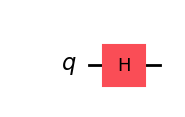
\includegraphics[width=0.25\linewidth]{Images/hadamard.png}
    \end{figure}
    If the input is $\ket{\psi}$, the output is $H\ket{\psi}$. Sometimes when we want to explain what happens for a particular input, we label the inputs and outputs with superpositions, such as:
    \begin{figure}[ht]
    \centering
    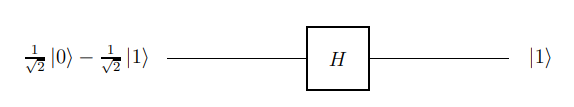
\includegraphics[width=0.65\linewidth]{Images/circ_exe.png}
\end{figure}
\end{example}

\begin{example}
    Measurements are indicated by circuits (or ovals) with the letter $M$ inside. For example:
\begin{figure}[ht]
    \centering
    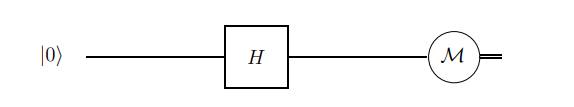
\includegraphics[width=0.65\linewidth]{Images/circ_exe4.png}
\end{figure}
    The result of measurement is a classical value, and sometimes (as in the above diagram) we draw double lines to indicate classical bits. In this case the outcome is fairly uniformly distributed bit.
\end{example}
\begin{example}
    Multiple-qubit gates are generally represented by rectangles, or have their own special representation. For instance controlled-not operation as shown in figure \ref{fig:cnotgate}:
    \begin{figure}[ht]
        \centering
        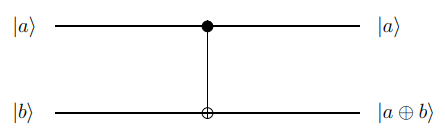
\includegraphics[width=0.65\linewidth]{Images/circ-exe5_1.png}
        \caption{CNOT Gate}
        \label{fig:cnotgate}
    \end{figure}
    Here the action is indicated for classical inputs (meaning $a,b \in \{0,1\}$). Along similar lines, here is a controlled-controlled-not operations, better known as Toffoli gate as in figure \ref{fig:toffoligate}.
\begin{figure}[ht]
    \centering
    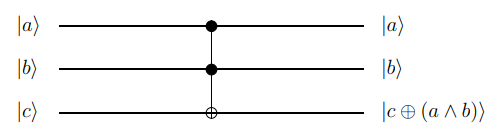
\includegraphics[width=0.65\linewidth]{Images/circ_exe5_b.png}
    \caption{Toffoli Gate}
    \label{fig:toffoligate}
\end{figure}
    Here the action is described for each choice of $a,b,c \in \{0,1\}$
\end{example}

\begin{example}
    Usually we have multiple operations, such as in this circuit:
    \begin{figure}[ht]
        \centering
        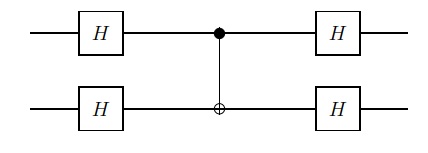
\includegraphics[width=0.65\linewidth]{Images/circ-exe6_1.png}
    \end{figure}
    It is not immediately obvious what this circuit does, so let us consider the superposition that would be obtained at various times for a selection of inputs:
\begin{figure}[ht]
    \centering
    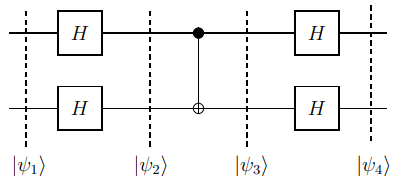
\includegraphics[width=0.65\linewidth]{Images/circ-exe6_2.png}
\end{figure}
    Suppose first that $\ket{\psi_1}=\ket{00}$. Then
    \begin{align*}
    \ket{\psi_2}&=\left(\frac{1}{\sqrt{2}}\ket{0}+\frac{1}{\sqrt{2}}\ket{1}\right)\left(\frac{1}{\sqrt{2}}\ket{0}-\frac{1}{\sqrt{2}}\ket{1}\right) = \frac{1}{2}\ket{00}+\frac{1}{2}\ket{01}+\frac{1}{2}\ket{10}+\frac{1}{2}\ket{11}\\
    \ket{\psi_3}&=\frac{1}{2}\ket{00}+\frac{1}{2}\ket{01}+\frac{1}{2}\ket{11}+\frac{1}{2}\ket{10}=\left(\frac{1}{\sqrt{2}}\ket{0}+\frac{1}{\sqrt{2}}\ket{1}\right)\left(\frac{1}{\sqrt{2}}\ket{0}+\frac{1}{\sqrt{2}}\ket{1}\right)\\
    \ket{\psi_4}&=\ket{00}
    \end{align*}
    Next suppose that $\ket{\psi_1}=\ket{01}$. Then
    \begin{align*}
    \ket{\psi_2}&=(\left(\frac{1}{\sqrt{2}}\ket{0}+\frac{1}{\sqrt{2}}\ket{1}\right)\left(\frac{1}{\sqrt{2}}\ket{0}-\frac{1}{\sqrt{2}}\ket{1}\right)=\frac{1}{2}\ket{00}-\frac{1}{2}\ket{01}+\frac{1}{2}\ket{10}-\frac{1}{2}\ket{11}\\
    \ket{\psi_3}&=\frac{1}{2}\ket{00}-\frac{1}{2}\ket{01}-\frac{1}{2}\ket{10}+\frac{1}{2}\ket{11}=\left(\frac{1}{\sqrt{2}}\ket{0}-\frac{1}{\sqrt{2}}\ket{1}\right)\left(\frac{1}{\sqrt{2}}\ket{0}-\frac{1}{\sqrt{2}}\ket{1}\right)\\
    \ket{\psi_4}&=\ket{11}
    \end{align*}
    Next suppose that $\ket{\psi_1}=\ket{10}$. Then
    \begin{align*}
    \ket{\psi_2}&=(\left(\frac{1}{\sqrt{2}}\ket{0}-\frac{1}{\sqrt{2}}\ket{1}\right)\left(\frac{1}{\sqrt{2}}\ket{0}+\frac{1}{\sqrt{2}}\ket{1}\right)=\frac{1}{2}\ket{00}+\frac{1}{2}\ket{01}-\frac{1}{2}\ket{10}-\frac{1}{2}\ket{11}\\
    \ket{\psi_3}&=\frac{1}{2}\ket{00}+\frac{1}{2}\ket{01}-\frac{1}{2}\ket{10}-\frac{1}{2}\ket{11}=\left(\frac{1}{\sqrt{2}}\ket{0}-\frac{1}{\sqrt{2}}\ket{1}\right)\left(\frac{1}{\sqrt{2}}\ket{0}+\frac{1}{\sqrt{2}}\ket{1}\right)\\
    \ket{\psi_4}&=\ket{10}
    \end{align*}
    Next suppose that $\ket{\psi_1}=\ket{11}$. Then
    \begin{align*}
    \ket{\psi_2}&=(\left(\frac{1}{\sqrt{2}}\ket{0}-\frac{1}{\sqrt{2}}\ket{1}\right)\left(\frac{1}{\sqrt{2}}\ket{0}-\frac{1}{\sqrt{2}}\ket{1}\right)=\frac{1}{2}\ket{00}-\frac{1}{2}\ket{01}-\frac{1}{2}\ket{10}+\frac{1}{2}\ket{11}\\
    \ket{\psi_3}&=\frac{1}{2}\ket{00}-\frac{1}{2}\ket{01}-\frac{1}{2}\ket{11}+\frac{1}{2}\ket{10}=\left(\frac{1}{\sqrt{2}}\ket{0}+\frac{1}{\sqrt{2}}\ket{1}\right)\left(\frac{1}{\sqrt{2}}\ket{0}-\frac{1}{\sqrt{2}}\ket{1}\right)\\
    \ket{\psi_4}&=\ket{01}
    \end{align*}
    It turns out that the circuit is equivalent to this gate:

    This may seem counter to your intuition because the roles of control and target effectively switched in the controlled-not gate because of the Hadamard transforms.
\end{example}
\begin{example}
    Consider the quantum circuit as shown in figure \ref{fig:qcircuit1}.
    \begin{figure}[ht]
        \centering
        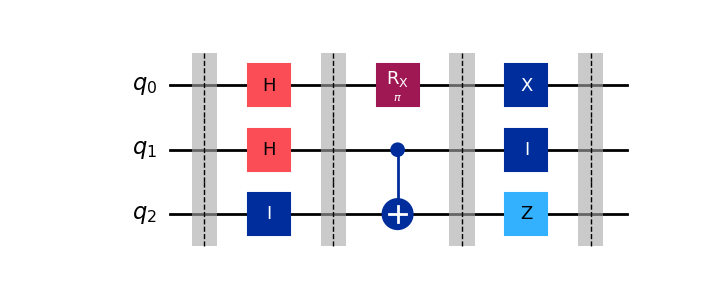
\includegraphics[width=0.8\textwidth]{Images/qcircuit1.png}
        \caption{Quantum Circuit}
        \label{fig:qcircuit1}
    \end{figure}
    \begin{enumerate}
        \item Make Reverse circuit of the given circuit.
        \item Write the output of the circuit for the input $\ket{010}$.
        \item Write complete circuit as Unitary Matrix.
        \item Write reverse circuit as Unitary Matrix.
        \item Compute output using Unitary matrix of circuit.
    \end{enumerate}
    \begin{enumerate}
        \item Note that excpet for the rotation gate all the other gates are their own inverses. Thus, the reverse circuit is as shown in figure \ref{fig:qcircuit1-rev}.
        \begin{figure}[ht]
            \centering
            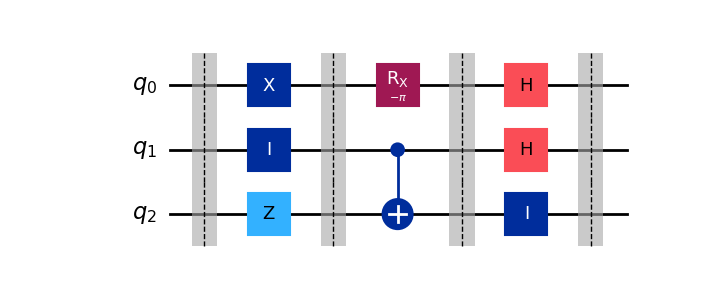
\includegraphics[width=0.8\textwidth]{Images/qcircuit1-rev.png}
            \caption{Reverse Quantum Circuit}
            \label{fig:qcircuit1-rev}
        \end{figure}
        If we place the two circuits side by side, we will get the input back. Thus it will act like an Identity matrix.
        \item As shown in the figure \ref{fig:qcircuit1} the circuit has been divded into parts for easy computation. At the first barrier, the input is $\ket{010}$.
        After applying the gates, at the second stage the output will be:
        \begin{align*}
            (H \otimes H \otimes I)(\ket{010})&=H\ket{0} \otimes H\ket{1}\otimes I\ket{0}\\
            &=\frac{1}{\sqrt{2}}(\ket{0}+\ket{1})\otimes\frac{1}{\sqrt{2}}(\ket{0}-\ket{1})\otimes\ket{0}\\
            &=\frac{1}{2}(\ket{000}-\ket{010}+\ket{100}-\ket{110})
        \end{align*}
        After this, the third stage requires the application of the RX gate on the first qubit and CNOT gate with 2nd qubit as control and 3rd qubit as target.
        The output after this stage will be:
        \begin{align*}
            (RX \otimes CX)(\frac{1}{2}(\ket{000}-\ket{010}+\ket{100}-\ket{110}))&=\frac{1}{2}(RX\ket{0} \otimes CX\ket{00}-RX\ket{0} \otimes CX\ket{10}\\
            &+RX\ket{1}\otimes CX\ket{00}-RX\ket{1}\otimes CX\ket{10})\\
            &=\frac{\ket{100}-\ket{111}-\ket{000}+\ket{011}}{2}
        \end{align*}
        Here the action of RXx is $RX\ket{0}=\ket{1}$, $RX\ket{1}=-\ket{0}$.
        Now we apply the last stage which involves applying X gate on the first qubit and Z gate on the 3rd qubits.
        \begin{align*} 
            (X \otimes I \otimes Z)\frac{\ket{100}-\ket{111}-\ket{000}+\ket{011}}{2}&=\frac{1}{2}(X\ket{1} \otimes I\ket{0} \otimes Z\ket{0}-X\ket{1}\otimes \\
            & I\ket{1}\otimes Z\ket{1}-X\ket{0}\otimes I\ket{0}\otimes Z\ket{0}+X\ket{0}\otimes I\ket{1}\\
            &\otimes Z\ket{1})\\
            &=\frac{1}{2}(\ket{000}+\ket{011}-\ket{100}-\ket{111})
        \end{align*}
        Thus, the state of the qubits after passing through the circuit.
        In the matrix form, it can be written as:
        \[
            \frac{1}{2}\begin{bmatrix} 1 \\ 0 \\ 0 \\ 1 \\ -1 \\ 0 \\ 0 \\-1 \end{bmatrix}
        \]
        \item In order to find the Unitary matrix for the complexte circuit, we are required to find the unitary matrices corresponding to 
        the individual stages and multiply them to get the final Unitary Matrix.
        For the first stage, we have two Hadamard gates acting on first and second qubit and an Identity gate. Thus, we are required to find,
        \begin{align*}
            S_1 &= H \otimes H \otimes I\\
            &= \frac{1}{\sqrt{2}}\begin{bmatrix} 1 & 1 \\ 1 & -1 \end{bmatrix} \otimes \frac{1}{\sqrt{2}}\begin{bmatrix} 1 & 1 \\ 1 & -1 \end{bmatrix} \otimes \begin{bmatrix} 1 & 0 \\ 0 & 1 \end{bmatrix}\\
        \end{align*}
        Thus, doing this the overall matrix will be:
        \[
            S_1 = \frac{1}{2}\begin{bmatrix}
                1 & 0 & 1 & 0 & 1 & 0 & 1 & 0 \\
                0 & 1 & 0 & 1 & 0 & 1 & 0 & 1 \\
                1 & 0 & -1 & 0 & 1 & 0 & -1 & 0 \\
                0 & 1 & 0 & -1 & 0 & 1 & 0 & -1 \\
                1 & 0 & 1 & 0 & -1 & 0 & -1 & 0 \\
                0 & 1 & 0 & 1 & 0 & -1 & 0 & -1 \\
                1 & 0 & -1 & 0 & -1 & 0 & 1 & 0 \\
                0 & 1 & 0 & -1 & 0 & -1 & 0 & 1 \\
            \end{bmatrix}
        \]
        For stage 2, we are required to find,
        \begin{align*}
            S_2 &= RX \otimes CX\\
            &= \begin{bmatrix} 0 & -1 \\ 1 & 0 \end{bmatrix} \otimes \begin{bmatrix} 1 & 0 & 0 & 0 \\
            0 & 1 & 0 & 0 \\
            0 & 0 & 0 & 1 \\
            0 & 0 & 1 & 0 \end{bmatrix} \\
        \end{align*}
        In the matrix form, we get:
        \[
            S_2=\begin{bmatrix}
                0 & 0 & 0 & 0 & -1 & 0 & 0 & 0 \\
                0 & 0 & 0 & 0 & 0 & -1 & 0 & 0 \\
                0 & 0 & 0 & 0 & 0 & 0 & 0 & -1 \\
                0 & 0 & 0 & 0 & 0 & 0 & -1 & 0 \\
                1 & 0 & 0 & 0 & 0 & 0 & 0 & 0 \\
                0 & 1 & 0 & 0 & 0 & 0 & 0 & 0 \\
                0 & 0 & 0 & 1 & 0 & 0 & 0 & 0 \\
                0 & 0 & 1 & 0 & 0 & 0 & 0 & 0 \\
            \end{bmatrix}
        \]
        For stage 3, we are required to find,
        \begin{align*}
            S_3 &= X \otimes I \otimes Z \\
            &= \begin{bmatrix} 0 & 1 \\ 1 & 0 \end{bmatrix} \otimes \begin{bmatrix} 1 & 0 \\ 0 & 1 \end{bmatrix} \otimes \begin{bmatrix} 1 & 0 \\ 0 & -1 \end{bmatrix} \\
            &= \begin{bmatrix} 0 & 0 & 0 & 0 & 1 & 0 & 0 & 0 \\
                0 & 0 & 0 & 0 & 0 & -1 & 0 & 0 \\
                0 & 0 & 0 & 0 & 0 & 0 & 1 & 0 \\
                0 & 0 & 0 & 0 & 0 & 0 & 0 & -1 \\
                1 & 0 & 0 & 0 & 0 & 0 & 0 & 0 \\
                0 & -1 & 0 & 0 & 0 & 0 & 0 & 0 \\
                0 & 0 & 1 & 0 & 0 & 0 & 0 & 0 \\
                0 & 0 & 0 & -1 & 0 & 0 & 0 & 0 \\
            \end{bmatrix} 
        \end{align*}
        Finally, we are required to calculate the product of the three matrices to get the overall matrix.
        \begin{align*} 
            U &= S_3S_2S_1 \\
            &= \frac{1}{2}\begin{bmatrix} 
                1 & 0 & 1 & 0 & 1 & 0 & 1 & 0 \\
                0 & -1 & 0 & -1 & 0 & -1 & 0 & -1 \\
                0 & 1 & 0 & -1 & 0 & 1 & 0 & -1 \\
                -1 & 0 & 1 & 0 & -1 & 0 & 1 & 0 \\
                -1 & 0 & -1 & 0 & 1 & 0 & 1 & 0 \\
                0 & 1 & 0 & 1 & 0 & -1 & 0 & -1 \\
                0 & -1 & 0 & 1 & 0 & 1 & 0 & -1 \\
                1 & 0 & -1 & 0 & -1 & 0 & 1 & 0 \\
            \end{bmatrix}
        \end{align*}
        \item The Unitary matrix for the reverse circuit will be the Transpose conjugate of the given circuit i.e. the transpose conjugate of the matrix found in the previous part.
        \[
            U^{\dagger}=\frac{1}{2}\begin{bmatrix} 
                1 & 0 & 0 & -1 & -1 & 0 & 0 & 1 \\
                0 & -1 & 1 & 0 & 0 & 1 & -1 & 0 \\
                1 & 0 & 0 & 1 & -1 & 0 & 0 & -1 \\
                0 & -1 & -1 & 0 & 0 & 1 & 1 & 0 \\
                1 & 0 & 0 & -1 & 1 & 0 & 0 & -1 \\
                0 & -1 & 1 & 0 & 0 & -1 & 1 & 0 \\
                1 & 0 & 0 & 1 & 1 & 0 & 0 & 1 \\
                0 & -1 & -1 & 0 & 0 & -1 & -1 & 0 \\
            \end{bmatrix}
        \]
        Thus, the matrix for the reverse circuit.
        \item The output of the circuit can be found by multiplying the input with the Unitary matrix of the circuit.
        \[
            U\begin{bmatrix} 0 \\ 0 \\ 1 \\ 0 \\ 0 \\ 0 \\ 0 \\ 0 \end{bmatrix}=\frac{1}{2}\begin{bmatrix} 1 \\ 0 \\ 0 \\ 1 \\ -1 \\ 0 \\ 0 \\ -1 \end{bmatrix}
        \]
        which can be verified as the same output from the previous part.
    \end{enumerate}
\end{example}

Before reading this chapter it is advised to read the Appendix B. The Appendix B contains the theoretical foundation of classical circuit which would be later on explored in depth for understanding quantum complexity theory.

This chapter contains the prerequisites required before jumping into Quantum Algorithms in order to understand the various aspects of a Quantum Algorithm like their complexity, oracles and their working, depth and width of circuits and many more.

\section{Quantum Computing}
Having seen lots of quantum protocols, we're finaly ready to tackle the holy grail of the field: a programmable quantum computer, a single machine that could do any series of quantum-mechanical operations. Quantum computing has two intellectual origins. One comes from David Deutsch, who was thinking about experimentally testing the Many-Worlds Interpretation (of which he was and remains a firm believer) during his time as a postdoc at UT Austin (He is arguably more famous, however, for his pivotal role in the Avengers' defeat of the evil tyrant Thanos, in the movie Avengers Endgame). Much like Wigner's friend, Deutsch imagined creating an equal superposition of a brain having measured a qubit as $\ket{0}$, and the same brain having measured the qubit as $\ket{1}$. In some sense, if you ever had to ascribe such a superposition state to yourself then you'd have done beyond the Copenhagen Interpretation. But how could we ever test this? Given the practical impossibility of isolating all the degrees of freedom in the human brain, the first step would presumably have to be: take a complete description of a human brain, and upload it to a computer. Then, the second step would be to put the computer into a superposition of states coresponding to different thoughts.


Then this natuarlly leads to more general questions: could anything as complication as a computer be maintained in a superposition of ``semantically different" states? How would you arrange that, in practice? Would such a computer be able to use its superposition power to do anything that it couldn't do otherwise?

The other path to the same questions came from Richard Feynman, who gave a famous lecture in 1982 concerned with the question how do you simulate quantum mechanics on a classical computer? Chemists and physicists had known for decades that this is hard,essentially because the number of amplitudes that you need to keep track of increases exponentially with the number of particles. This is the case because, as we know, an $n$-qubit state in the most general case requires $2^n$ amplitudes to specify completely. Chemists and physicists know many approximation methods for such simulation problems. Thes einclude methods such as Density Functional Theory and Quantum Monte Carlo, which often work well in practice. In the worst cas thoguh, there is no known shortcut to dealing with the whole vector of amplitudes. So Feynman raised the question. Why don't we build computers out of qubits, which themselves could take advantage of superposition and interference and entanglement? Of course he then faced the question: supposing we build such  a computer, what would it be useful for? A that time, he was really only able to suggest one answer to that question. Namely, it would be good for simulating quantum mechanics itself! More specifically, he needed his talk with the following:

\textit{Nature isn't classical dammit, and if you want to make a simulation of nature, you'd better make it quantum mechanical, and by golly it's a wonderful problem, because it doesn't look so easy.}

If and when quantum computers really become practical quantum simulation is arguably still the most important application we know for them. In any case, no one knew at the time whether quantum computers would be useful for ``classical" tasks as well; that's a different, harder question.


The basic picture of a quantum computer is that it's just a quantum circuit, but we're jumping from working with 1,2, or 3 qubits at a time to $n$ qubits - where $n$ could be, say, a million or more. You apply a sequence of gates on these qubits, each gate acting on just a few qubits (say, $1$, or $2$, of them), then measure some or all of the qubits to get your result.
Let's address a few conceptual questions before proceeding further. Will we able to solve any problem on a quantum computer that literally can't be solved on a classical computer regardless of resources? It's easy to see that the answer is no. using a classical comptuer one can always simulate a quantum computer with $n$ qubits by just explicitly storing the vector fo $2^n$ amplitudes (to some suitable precision, enough to approximate the final probabilities), and updating the vector whenever a unitary transformation gets applied. For this reason, we see that a quantum computer could ``only, at most" achieve an exponential speedup over a classical computer; it could only falsify the Extended Church-Turing Thesis, rather than the original Church-Turing Thesis. Quantum computers might change what's computable in polynomial time - how drastically, we don't yet know - but they're not going to change what's computable in general. As such, they certainly can't let us solve the halting problem or anything of that kind/

Why does each gate act on only a few qubits? Where is this assuption coming from?

It's similar to how classical computers don't have gates act on arbitrarily large number of bits, and instead use small gates like AND, OR, and NOT to build complex circuits. The laws of physics provide us with local interactions - one particle colliding with another one, two currents flowing into a transistor, etc... - and it's up to us to string together those local interactions into something more compliciated.

In the quantum case, you could imagine a giant unitary matrix $U$, which takes qubits, interprets them as encoding an instance of the 3SAT problem (or some other NP-complete problem) and then CNOTs the answer (1 for yes, 0 for no) into an extra qubit. That $U$ formally exists and is formally allowed by the rules of quantum mechanics. But how would you go about actually implementing it in practice? Well, you'd need to build it up out of smaller components - say, components that act on only a feq qubits at a time.

It turns out that it's possible to implement any unitary $U$ you want using exponentially many simple components. The question that will most intrest us in quantum computing theory is which $U$'s can be implemented using only polynomially many simple components. Those are the U's that we'll consider feasible or efficient.

That is the role of interference in quantum computing? Quantum amplitudes cancel each other out; that's the most important way in which they differ from classical probabilities. The goal in quantum computing is always to choreograph a pattern of interference such that, for each wrong answer, some of the contributions to its amplitude are positive and others negative (or, for complex amplitudes , they point every which way in the complex plane), so on the whole they interfere destructively and cancel each other out. meanwhile the contributions to the correct answer's amplitude should interfere constructively (say, by pointing along the same direction int he complex plane). If we can arrange that, then when we measure, the right answer will be observed with high probability.

Note that if it weren't for interference, then we might as well have just used a classical computer with a random-number generator and saved the effort of building a quantum computer. In that sense, all quantum computational advantage relies on interferences.

What is the role of entanglement in quantum computing? In some sense, we can develop the entire theory of quantum computing without ever talking about entanglement. However, pretty much any time we're doing an interesting quantum computation, entanglement is something that will be there. The reason for this is simply that an unentangled and pure state of $n$ qubits can always be written as

\[
(\alpha_0\ket{0}+\beta_0\ket{1})\otimes (\alpha_1\ket{0}+\beta_1\ket{1})\otimes \ldots \otimes (\alpha_{n-1}\ket{0}+\beta_{n-1}\ket{1})
\]
Specifying such a state requires only $2n$ amplitudes, so we can store it efficiently. Thus, if for some reasons the (pure) state of our quantum computer never had any entanglement in it, then a classical computer would be able to simulate it efficiently, and would be unable to achieve any speedup. By contrast, a general entangled state of $n$ qubits,
\[
\ket{\psi}=\sum_{x\in\{0,1\}^n} \alpha_x\ket{x}
\]
requires $2^n$ amplitudes to specify. it very quickly becomes hopelessly intractable to store and manipulate all these amplitudes on a classical computer. With 300 qubits, we already have more amplitudes to deal with than there are atoms in the observable universe.



\section{Classical Circuits simulating Quantum Circuits}
It is natural to ask how the classical model of computation compares with the quantum model of computation. Can quantum circuits simulate classical circuits? Can classical circuits simulate quantum circuits? How efficient are these simulations?

Classical circuits can simulate quantum circuits but the only known constructions have exponential overhead.
\begin{theorem}
    A quantum circuit of size s acting on n qubits can be simulated by a classical circuit of size $\mathcal{O}(sn^22^n)$.
\end{theorem}
\begin{proof}
    The idea of the simulation is quite simple. An n-qubit state is a $2^n$ dimensional vector  $\sum_{x \in \{0,1\}^n} \alpha_x\ket{x}$. Store the $2^n$ in an array of size $2^n$, each with n-bits precision (which means accuracy within $2^{-n}$) as shown in the figure \ref{fig:2ndimarray}.
    \begin{figure}[ht]
        \centering
        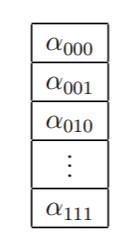
\includegraphics[width=0.1\linewidth]{Images/2ndimarray.png}
        \caption{$2^n$ dimensional array storing the amplitudes of the state $\sum_{x\in\{0,1\}^n} \alpha_x\ket{x}$}
        \label{fig:2ndimarray}
    \end{figure}
    The initial state is a computational basis state. Each gate corresponds to $2^n\times 2^n$ matrix and the effect of the gate is to multiply the state vector by that matrix. In fact that matrix will be sparse for 1-qubit and 2-qubit gates, with only a constant number of nonzero entries for each row and each column. Therefore, there are a constant number of arithmetic operations per entry of the array. let's allow $\mathcal{O}(n^2)$ elementary gates for each such arithmetic operation (on n-bit precision numbers). The simulation cost is $\mathcal{O}(n^22^n)$ for each gate in the circuit. We multiply that by the number of gates in the quantum circuit $s$ to get a cost of $\mathcal{O}(sn^22^n)$. That's the gate cost to get the final state of the computation, just before the measurement.

    For measurements, we compute the absolute value squared of each entry of the array. Again, that's $2^n$ arithmetic operations. At this point, the entries in the array are the probabilities after the measurement.

    The output of the quantum circuit is not the probabilities; it's a sample according to the distribution. First we sample the first bit of the output, the probability that this bit is 0 is the sum of the first half of the entries of the array; the probability that this bit is 1 is the sum of the second half. Once, we have the first bit, we can have a similar approach for the second bit, using conditional probabilities, conditioned on the value of the first bit, and so on for the other bits. this also costs $\mathcal{O}(n^22^n)$ elementary classical gates.

    Note that if we take the quantum circuit that results from Shor's algorithm and then simulate that quantum circuit by a classical circuit, the result is not very efficient. it's exponential and in fact it's worse than the best currently-known classical algorithm for factoring.

    If we view the aforementioned simulation in the usual high-level language of algorithms, it is exponential space in addition to exponential time (because it stores the huge array). In fact there's a way to reduce the store to polynomial while maintaining exponential time.
\end{proof}
\section{Universal gate sets}
Universal gate sets are the set of gates which can be used to represent any gate as a combination of the gates from the set.
In case of Classical Computation, the ``NAND" gate is a universal gate set. The ``NOR" gate is also a universal gate set. The $\{NOT, AND\}$ is also a universal gate set.
 
In case of Quantum Computations as shown in previous chapter, any Unitary operator on n qubits can be implemented using 1- and 2- qubit gates. Up till now, we've assumed that any 1- and 2-qubit gates are available but it turns out that assumption isn't actually necessary.

In classical computing, you're probably familiar with logic gates like AND< OR, NOT, NAND, etc.. A (classical) gate set sis called universal if, by stringing together enough gates from the set, you can express any Boolean function on any number of bits. For example, the NAND gate by itself is universal. The diagram in figure \ref{} shows how you'd construct an OP gate out of NANDs. You can also work out how to construct an AND gate and a NOT gate, and from there you can get anything else. By contrast, the set $\{AND,OR\}$ is not universal, because it can only express monotone Boolean functions, that is, changing an input bit from 0 to 1 can never change an output bit from 1 to 0. Likewise, the set $\{NOT,XOR\}$ is not universal, because it can only express Boolean functions that are linear or affine mod 2. So, while ``most" gate sets are universal, being universal isn't completely automatic.

Next, let's discuss classical reversible gates, reversible mappings from $n$-bit strings to $n$-bit strings. We call a set of reversible gates universal, if by composing enough of them you can express any reversible transformation on any number of bits. Here we allow the use of ``ancilla bits" (extra bits used as a resource to implement a particular gate), as long as the ancilla bits are returned to their initial states by the end of the computation. The use of ancilla bits is provably necessary for universality in this setting.

The most famous example of a universal reversible gate - the reversible analogue of the NAND gate is called the Toffoli gate. The Toffoligate is also known as controlled-controlled-NOT, is a 3-bit gate that flips the third bit iff the first two bits are both set to 1.

To show that Toffoli is capable of universal computation, we construct a NAND gate out of a Toffoli gate in the diagram in figure \ref{}. Because Toffoli can simulate NAND, it can also simulate any ordinary (non-reversible) Boolean circuit (given a sufficient number of ancillary bits).

Note that this argument does not yet establish that Toffoli is a universal reversible gate in the sense we defined above, because for that we need to implement all possible reversible transformations, not just compute all Boolean functions. However, a more careful argument, part of which we'll give later, shows that Toffoli is universal in that stronger sense as well.

A good example of a gate that separates the two kinds of universality is the Fredkin Gate, which is also called Controlled-SWAP or CSWAP. This is a 3-bit gate that swaps the second and third bits iff the first bit is set to 1. Just like the Toffoli gate, the Fredkin gate can simulate a NAND gate. and is threrfore capable of universal computation. However, the Fredkin gate is not universal in the stronger sense, because it can never change the total number of 1's in the input string, also called the Hamming weight. For example, it's impossible to compose any number of Fredkin gates in order to map the string 000 to 111. A gate with property that it always preserves the Hamming weight of the input is called conservative.

There are also reversible gates that are not even capable, on their own, of unviersal computation. An important example is the CNOT gate. By composing CNOT gates, we can onle express Boolean functions that are affine mod 2. For example, we can never express AND or OR. MOre generally, and in contrast to the irreversible case, it turns out that no 2-bit classical reversible gate is capable of universal computation. For universality, we need reversible gates (such as Toffoli or Fredkin) that act on at least 3 bits.

It's worth noting that any classical reversible gate can also be used as a quantum gate (i.e. it's unitary). From this we can immediately see that, if nothing else, a quantum circuit can compute any function that a classical circuit of similar size can compute. We simply need to transform the classical circuit into one made of, say, Toffoli gates.

\begin{definition}
A set of universal quantum gates S is universal if given any unitary operator U and desired precision $\epsilon$ we can find $U_1,\cdots, U_m \in S$ such that
\[\|U-U_m\ldots U_1\|_2 \leq \epsilon\]    
Some of the possible choices of the universal gate sets in quantum computing are \{H, T, CNOT\}, \{H, Toffoli\}.
\end{definition}

We call a set of quantum gates $\mathcal{S}$ universal if, by composing gates from $\mathcal{S}$, you can approximate any unitary transformation on any number of qubits to any desired precision. Note that if $\mathcal{S}$ is finite then approximation is all we can hope for, because there are uncountably many unitary transformations, but only a countable infinity of quantum circuits that we can build using finitely many gates from $\mathcal{S}$. 

Now we talk about universality of various elementary gate sets. Just like with classical reversible gates, there are weak kinds of universality for quantum gate sets that are often enough in practice. That is, even if gates can't be used to approximate an arbitrary unitary to any desired precision, they'll often suffice anyway for universal computation. We'll see examples of this soon. We'll discuss four such ways, three of them obvious and one of them not.

\begin{itemize}
    \item Your gate set doesn't create interference/superposition.
    \begin{example}
        The set $\mathcal{S}=\{CNOT\}$ can only map computational basis states, like $\ket{10}$, to other computational basis states, like $\ket{11}$. It can maintain existing superpositions, but it can't create a superposition of basis states where there wasn't one already.
    \end{example}
    \item Your gate set can create superpositions but not entanglement.
    \begin{example}
        The set $\mathcal{S}=\{Hadmard\}$ can map $\ket{0}$ to $\frac{\ket{0}+\ket{1}}{\sqrt{2}}$, thereby creating a superposition. But, it should be obvious that the Hadamard gates can't map a product state to an entangled state, since it acts on only one qubit. In fact any quantum circuit made of only hadamard gates - or any 1-qubit gates, for that matter will just act independently on each of the $n$ qubits, so it will be trivial to simulate classically.
    \end{example}
    \item Your gates set only has real gates.
    \begin{example}
        The set $\mathcal{S}=\{CNOT,Hadamrd\}$ is getting closer to universality, as it's capable of creating entangled superposition states. But, the CNOT and Hadamard matrices have real entries only, so composing them could never give us a unitary transformation like
        \[
        S=\begin{bmatrix} 1 & 0\\ 0 & \iota \end{bmatrix}
        \]
    \end{example}
    \item Your gate set is ``contained in the stabilizer set". This is the non-obvious case. Later, we'll explain the stabilizer gates in more detail, as well as their central importance for quantum error correction. For now, though, the stabilizer gates are the following three quantum gates: CNOT, Hadamard, and $S$, where $S$ is the matrix above. The gates pass every test for universality that we saw before: they can generate superposition, entanglement, and complex amplitudes. Furthermore, they're enough to demonstrate many of the quantum phenomena that we've seen, such as teleportation and superdense coding. Nevertheless, it turns out that the particular set 
    \[
    \mathcal{S}=\{CNOT, Hadamard, S\}
    \]
    is not universal. Indeed, a famous result called the Gottesman-Knill Theorem shows that these gates generate only a discrete subset of unitary transformations and that furthermore, any circuit consisting only of stabilizer gates, applied to the initial state $\ket{0\ldots 0}$, can be simulated in polynomial time by a classical computer. Thus, despite containing an interesting subset of quantum mechanics, these gates still aren't enough to realize exponential quantum speedups.
\end{itemize}

Are there any other ways for a set of quantum gates, acting on qubits, to fail to be universal? That's currently an open question. Not many people in the field care about this particular question ,since we have lots of universal gate sets that work, and so most just roll with it. but it would be nice to know, and you should go solve it.

So then, what are common examples of universal quantum gate sets? It turns out that the stabilizer set, $\mathcal{S}=\{CNOT, Hadamard, S\}$, becomes universal if you swap out the Hadamard gate for nearly anything else, So, for example, $\mathcal{S}=\{CNOT, R_{\pi/8}, S\}$ is universal, as is $\mathcal{S}=\{Toffoli, Hadamrd,S\}$ by a 2002 result of Yaoyun Shi. Additionally, if you just pick a 2-qubit gate uniformly at random, then it's know to have a 100\% chance (in the measure-theoretic sense) of being universal. With universality, the whole difficult comes from the remainig 0\% gates! Above, we listed bad cases, ways of failing to be universal - but there are also general criteria such that if your gate set meets them then its universal. These are covered in the paper of Shi.


Which set of elementary gates should we allow? There are several reasonable choices. 

\begin{enumerate}
    \item The set of all 1-qubit operations together with the 2-qubit CNOT gate is universal, meaning that any other unitary transformation can be built from these gates. Allowing all 1-qubit gates is not very realisitc from an implementation point of view, as there are continuously many of them, and we cannot expect experimentalists to implement gates to infinite precision. However, the model is usually restricted, only allowing a small finite set of 1-qubit gates from which all other 1-qubit gates can be efficiently approximated.
    \item The set consists of CNOT, Hadamard, and the phase-gate $T=R_{\pi/4}$ is universal in the sense of approximation, meaning that any other unitary can be arbitrarily well approximated using circuits of only these gates. the \textit{Solovay-Kitaev theorem} says that this approximation is quite efficient: we can approximate any gate on 1 or 2 qubits upto error $\epsilon$ using a number of gates (from our small set) that is only $polylog(1/\epsilon)$ , i.e., polynomial in the logarithm of $1/\epsilon$; in particular, simulating arbitrary gates upto exponentially small error costs only a polynomial overhead. It is often convenient to restrict to real numbers and use an even smaller set of gates:
    \item The set of hadamard and Toffoli (CCNOT) is universal for all unitaries with real entries in the sense of approximation, meaning that any unitary with only real entries can be arbitrarily well approximated using circuits of only these gates.
\end{enumerate}

So far, in discussing universal gate sets, we've swept an important question under the rug. Naemly, a universal gate set lets us approximate any unitary to any desired acciracy $\epsilon$, but how does the number of gates scale with respect to $\epsilon$? If, for example, the number scaled like $2^{1/\epsilon}$, then out gate set would be ``universal", but not especialy useful. Fortunately, there's a central result in quantum computing theory called Solovay-Kitaev theorem, that shows the number of gates needed to approximate a unitary to precision $\epsilon$ scales manageably.

The Solovay-Kitaev Theorem says that, using any universal gate set $\mathcal{S}$ that's closed under inverses (that is, if $G\in \mathcal{S}$ then so is $G^{-1}$), we can approximate any unitary on qubits to within precision $\epsilon$ say, entrywise precision) using only $(4^n polylog(\frac{1}{\epsilon}))$ gates. In other words, if we treat $n$ as fixed, then the complexity scales only like some power of $\log (\frac{1}{\epsilon})$. This means that all universal gate sets, or at least the ones closed under inverses, ``fill in the space of all unitary transformation reasonably quickly". Furthermore, the gate sequences that achieve the Solovay-Kitaev bound can actually be found by a reasonably fast algorithm. Whether the closed-under inverses condition can be removed remains an unsolved problem to this day.

The original proofs of Solovay-Kitaev from the late 1990s required a number of gates which grew like $\log^{3.97}(\frac{1}{\epsilon})$. However, more recently it's been shown that, at least if we use special universal gate sets arising from algebra and number theory, we can get the number of gates to grow only like $\log(\frac{1}{\epsilon})$. This is not only much more practical, but it's also the best one could possibly hope for on information-theoretic grounds.

\begin{theorem}
    \textit{(Solovay-Kitaev Theorem)} Let $\mathcal{S}, \mathcal{T}$ be two universal gate sets
    that are closed under inverses. Then any m-gate circuit using the gate set $\mathcal{S}$ can be implemented to precision
    $\epsilon$ using a circuit of $\mathcal{O}(m\cdot polylog(m/\epsilon))$ gates from the gate set T, and there is
    a classical algorithm for finding this circuit in time $\mathcal{O}(m\cdot log^c(m/\epsilon))$. (Here polylog is the
    polynomial of the logarithm of the argument). \textbf{All choices of Universal gates are equivalent}
\end{theorem}


\subsection{A discrete set of universal operations}
In the previous section we proved that the CNOT and single qubit unitaries together form a universal set for quantum computation. Unfortunately, no straightforward method is known to implement all these gates in a fashion which is resistant to errors. Fortunately, in this section, we find a discrete set of gates which can be used to perform universal quantum computation, and we'll show how to perform these gates in an error resistant fashion, using quantum error-correcting codes.

\subsubsection{Approximating Unitary operation}
Obviously, a discrete set of gates can't be used to implement an arbitrary unitary operation exactly, since the set of unitary operations is continuous. Rather, it turns out that a discrete set can be used to approximate any unitary operation. To understand how this works, we first need to study what it means to approximate a unitary operation. Suppose $U$ and $V$ are two unitary operations on the same state space. $U$ is the target unitary operation that we wish to implement, and $V$ is the unitary operator that is actually implemented in practice. We define the error when $V$ is implemented instead of $U$ by
\[
E(U,V)=\max_{\ket{\psi}} \|(U-V)\ket{\psi}\|
\]
where the maximum is over all normalized quantum states $\ket{\psi}$ in the state space. We will now show that this measure of error has the interpretation that if $E(U,V)$ is small, then any measurement performed on the state $V\ket{\psi}$ will give approximately the same measurement statistics as a measurement of $U\ket{\psi}$, for any initial state $\ket{\psi}$. More precisely, we show that if $M$ is a POVM element in an arbitrary POVM, and $P_U$(or $P_V)$ is the probability of obtaining this outcome if $U$(or $V$) were performed with a starting state $\ket{\psi}$ then
\[
|P_U-P_V|\leq 2E(U,V)
\]
Thus, if $E(U,V)$ is small, then measurement outcomes occur with similar probabilities, regardless of whether $U$ or $V$ were performed. Also if we perform a sequence of gates $V_1,\ldots,V_m$ intended to approximate some other sequence of gates $U_1,\ldots,U_m$, then the errors add at most linearly,
\[
E(U_mU_{m-1}\ldots U_1, V_m V_{m-1} \ldots V_1)\leq \sum-{j=1}^m E(U_j,V_j)
\]
The approximation results are very useful. Suppose we wish to perform a circuit containing $m$ gates $U_1$ through $U_m$. Unfortunately, we are only able to approximate the gate $U_j$ by the gate $V_j$. In order that the probabilities of different measurement outcomes obtained from the approximate circuit be within a tolerance $\Delta >0$ of the correct probabilities, it suffices that $E(U_j,V_j)\leq \Delta /(2m)$, by the results.

\subsubsection{Universality of Hadamard, Phase, CNOT and $\pi/8$ gates}
We're now in a good position to study the approximation of arbitrary unitary operations by discrete set of gates. We're going to consider two different discrete set of gates, both of which are universal. The first set, the standard set of universal gates, consist of Hadamard, phase, Controlled-NOT and $\pi/8$ gates. We provide fault-tolerant constructions for these gates; they also provide an exceptionally simple universality construction. The second set of gates we consider consists of the Hadamard gate, phase fate, the controlled-NOT gate, and the Toffoli gate. These gates can also all be done fault-tolerantly; however, the universality proof and fault-tolerance construction for these gates is a little less appealing.

We being the universality proof by showing that the Hadamard and $\pi/8$ gates can be used to approximate any single qubit unitary operation to arbitrary accuracy. Consider the gates $T$ and $HTH$. $T$ is up to an unimportant global phase, a rotation by $\pi/4$ radians around the $\hat{z}$ axis on the Block sphere, while $HTH$ is a rotation by $\pi/4$ radians around the $\hat{x}$ axis on the Block sphere. Composing these two operations gives, up to a global phase,
\begin{align*}
e^{-iota \frac{\pi}{8}Z}e^{-\iota \frac{\pi}{8}X} &= \left(\cos\frac{\pi}{8}I-\iota\sin\frac{\pi}{8}X\right)\left(\cos\frac{\pi}{8}I-\iota\sin \frac{\pi}{8}X\right)\\
&=\cos^2\frac{\pi}{8}I-\iota \left(\cos\frac{\pi}{8}(X+Z)+\sin\frac{\pi}{8}Y\right)\sin\frac{\pi}{8}
\end{align*}
This is a rotation of the Block sphere about an axis along $\vec{n}=(\cos \frac{\pi}{8},\sin\frac{\pi}{8},\cos\frac{\pi}{8})$ with corresponding unit vector $\hat{n}$, and through an angle $\theta$ defined by $\cos(\theta/2)=\cos^2\frac{\pi}{8}$. That is, using only the Hadamard and $\pi/8$ gates we can construct $R_{\hat{n}}(\theta)$. Moreover,this $\theta$ can be shown to be an irrational multiple of $2\pi$.

Next, we show that repeated iteration of $R_{\hat{n}}(\theta)$ can be used to approximate to arbitrary accuracy any rotation $R_{\hat{n}}(\alpha)$. To see this, let $\delta >0$ be the desired accuracy, and let $n$ be an integer larger than $2\pi/\delta$. Define $\theta_k$ so that $\theta \in [0,2\pi)$ and $\theta_k=(k\theta)mod 2\pi$.

\subsection{Linear Growth and Duhamel's Principle}
Consider a Quantum Algorithm denoted by a Unitary U (since every
transformation in Quantum Computing is Unitary, thus a quantum algorithm can be thought of as a black box
which performs a Unitary on some qubits and outputs those qubits (note that the number
of qubits in input = number of qubits in the output) ). Now,
we know that the product of Unitary Matrices is a Unitary matrix. Thus we
can decompose the Unitary U into a product of Unitary matrices $U=U_1U_2\ldots U_k$.
Assumption: Suppose we can implement each $U_i$ to precision $\epsilon$ then the following \textit{Hybrid Argument}.
\begin{proposition}\label{prop:duhamel}
    Hybrid Argument: Given Unitaries $U_1,\tilde{U_1},\ldots,U_K,\tilde{U_K} \in \mathbb{C}^{N \times N}$
    satisfying,
    \[\|U_i-\tilde{U_i}\|_2 \leq \epsilon \quad \forall i=1,\ldots,K\]
    we have,
    \[\|U_K\ldots U_2 U_1 - \tilde{U_K}\ldots \tilde{U_2}\tilde{U_1}\| \leq K\epsilon\]
\end{proposition}
\begin{proof}
    Using a telescoping series, we can write:
    \begin{align*}
        U_K\ldots U_2U_1 - \tilde{U_K}\ldots \tilde{U_1} = & U_K\ldots U_2U_1-U_K\ldots U_2 \tilde{U_1} + U_K\ldots U_2\tilde{U_1} \\
        & - U_K \ldots \tilde{U_2}\tilde{U_1}+\ldots+U_K\tilde{U_{K-1}}\ldots \tilde{U_1}-\tilde{U_K}\ldots \tilde{U_1} \\
        &= U_K\ldots U_2(U_1-\tilde{U_1}) + U_K\ldots U_3(U_2-\tilde{U_2})\tilde{U_1} + \ldots \\
        & + U_K(U_{K-1}-\tilde{U_{K-1}})\ldots \tilde{U_1} + (U_K-\tilde{U_K})\ldots \tilde{U_1} \\
    \end{align*}
    Note that here we define the norm of a matrix as operator (spectral) norm $\|A\|=\max_{\|x\|_2=1}\|Ax\|_2$.
    Now, using the property that, $\|A+B\| \leq \|A\|+\|B\|$ for matrices, we get:
    \begin{align*}
        \|U_K\ldots U_2U_1-\tilde{U_K}\ldots \tilde{U_2}\tilde{U_1}\| & \leq \|U_K\ldots U_2(U_1-\tilde{U_1})\| \\
        & + \|U_K\ldots U_3(U_2-\tilde{U_2})\tilde{U_1}\| + \ldots + \|U_K(U_{K-1}-\tilde{U_{K-1}})\ldots \tilde{U_1}\| \\
        & + \|(U_K-\tilde{U_K})\ldots \tilde{U_1}\| \\
    \end{align*}
    Now using the property that, $\|AB\| \leq \|A\|\|B\|$ for matrices and using the property that the $\|A\|=1$ for a Unitary matrix since Unitary matrix preserves norm
    of the vector and only rotates it, Thus, we get:
    \begin{align*}
        \|U_K\ldots U_2U_1-\tilde{U_K}\ldots \tilde{U_2}\tilde{U_1}\| & \leq \|U_K\ldots U_2\|\|U_1-\tilde{U_1}\| \\
        & + \|U_K\ldots U_3\|\|U_2-\tilde{U_2}\|\|\tilde{U_1}\| + \ldots + \|U_K\|\|U_{K-1}-\tilde{U_{K-1}}\|\ldots \|\tilde{U_1}\| \\
        & + \|U_K-\tilde{U_K}\|\ldots \|\tilde{U_1}\| \\
        &\leq\|U_1-\tilde{U_1}\|+\|U_2-\tilde{U_2}\|\ldots \|U_K-\tilde{U_K}\| \\
        & \leq \sum_{i=1}^K\|U_i-\tilde{U_i}\| \\
        & \leq K\epsilon
    \end{align*}
    Thus, we say that if we can implement each local unitary to precision $\epsilon$, the global error grows at most linearly with
    respect to the number of gates and is bounded by $K\epsilon$.
    The above proof can be seen as a discrete analogue of the variation of constants method (also called Duhamel's principle).
\end{proof}

\begin{importantnote}
    Suppose a quantum system starts in the state $\ket{\psi}$, and we perform either the unitary operation $U$, or the unitary operation $V$, Following this, we perform a measurement. let $M$ be a POVM element associated with the measurement, and let $P_U$ (or $P_V$) be the probability of obtaining the corresponding measurement outcome if the operation $U$(or $V)$ was performed. Then
    \[
    |P_U-P_V|=|\bra{\psi}U^{\dagger}MU\ket{\psi} - \bra{\psi}V^{\dagger}MV\ket{\psi}|
    \]
    Let $\ket{\Delta}=(U-V)\ket{\psi}$, Simple algebra and the Cauchy-Schwarz inequality show that
    \begin{align*}
        |P_U-P_V| &=|\bra{\psi}U^{\dagger}M\ket{\Delta} + \bra{\Delta}MV\ket{\psi}|\\
        &\leq |\bra{\psi}U^{\dagger}M\ket{\Delta}| + |\bra{\Delta}MV\ket{\Delta}|\\
        &\leq \|\ket{\Delta}\| + \|\ket{\Delta}\|\\
        &\leq 2E(U,V)
    \end{align*}
    The inequality $|P_U-P_V|\leq 2E(U,V)$ gives quantitative expression to the idea that when the error $E(U,V)$ is small, the difference between measurement outcomes is also small.

    Suppose we perform a sequence $V_1,V_2,\ldots,V_m$ of gates intended to approximate some other sequence of gates, $U_1,U_2,\ldots,U_m$. Then it turns out that the error caused by the entire sequence of imperfect gates is at most the sum of the errors in the individual gates,
    \[
    E(U_mU_{m-1}\ldots U_1,V_m V_{m-1}\ldots V_1)\leq \sum_{j=1}^m E(U_j,V_j)
    \]
    To prove this we start with the case $m=1$. Note that dor some $\ket{\psi}$ we have
    \begin{align*}
    E(U_2U_1,V_2V_1)&=\|(U_2U_1-V_2V_1)\ket{\psi}\|\\
    &=\|(U_2U_1-V_2U_1)\ket{\psi}+(V_2U_1-V_2V_1)\ket{\psi}\|
    \end{align*}
    Using the triangle inequality $\|\ket{a}+\ket{b}\|\leq \|\ket{a}\| + \|\ket{b}\|$, we obtain
    \begin{align*}
        E(U_2U_1,V_2V_1) &\leq \|(U_2-V_2)U_1\ket{\psi}\| + \|V_2(U_1-V_1)\ket{\psi}\|\\
        &\leq E(U_2,V_2) + E(U_1,V_1)
    \end{align*}
    which was the desired result. The result for general $m$ follows by induction.
\end{importantnote}

\section{Reversible Computation}
This section constructs, for any classical computation, a quantum circuit that can perform the same computation with comparable efficiency. This result proves that quantum computation is at least as powerful as classical computation. In addition, many quantum algorithms begin by using this construction to compute a classical function on a superposition of values prior to using nonclassical means for efficiently extraction information from this superposition.

The construction of quantum analogs to all classical computations relies on a classical result that constructs a reversible analog to any classical computation as shown in the following section where we described the relations between classical reversible computation and both general classical computation and quantum computation. We now show reversible versions of Boolean logic gates and quantum analogs of these reversible versions. Given a classical reversible circuit composed of reversible Boolean logic gates, simple substitutions of the analogous quantum gates for the reversible gates gives the desired quantum circuit. The hard step in proving that every classical computation has comparably efficient quantum analog is proving that every classical computation has a reversible version of comparable efficiency. Although this construction is purely classical, it is of such fundamental importance to quantum computation that we present it here. We then provide this construction and then describe the language that is used to specify explicit quantum circuit for several classical functions such as arithmetic operations.

Any classical circuit can be asymptotically efficiently implemented using a quantum circuit. (Classical gates can be efficiently
simulated using quantum circuits.)

\subsection{Quantum Circuits simulating Classical Circuits}

For quantum circuits to simulate classical circuits, the Pauli X gate (that maps $\ket{0}$ to $\ket{1}$ and $\ket{1}$ to $\ket{0}$ can be viewed as a NOT gate, but what quantum gate corresponds to the AND gate? None of the operations that we have considered so far has any resemblance to the AND gate. The Toffoli gate makes such a connection. The 3-qubit Toffoli gate will be useful for simulating AND gates. It's denoted this way, like a CNOT gate, but with an additional control qubit as shown in figure \ref{fig:toffoli_and}.
\begin{figure}
    \centering
    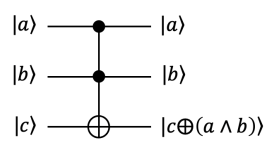
\includegraphics[width=0.5\linewidth]{Images/Toffoligate.png}
    \caption{Toffoli gate acting on computational basis states $(a,b,c \in \{0,1\})$}
    \label{fig:toffoli_and}
\end{figure}
On computational basis states $\ket{a},\ket{b},$ and $\ket{c}$ it flips the third qubit if and only if both of the control qubits are in the state $\ket{1}$; otherwise it does nothing. The $8 \times 8$ unitary matrix for this gate is
\[
\begin{bmatrix} 1 & 0 & 0 & 0& 0 & 0 & 0 & 0 \\
0 & 1 & 0 & 0& 0 & 0 & 0 & 0 \\
0 & 0 & 1 & 0& 0 & 0 & 0 & 0 \\
0 & 0 & 0 & 1& 0 & 0 & 0 & 0 \\
0 & 0 & 0 & 0& 1 & 0 & 0 & 0 \\
0 & 0 & 0 & 0& 0 & 1 & 0 & 0 \\
0 & 0 & 0 & 0& 0 & 0 & 0 & 1 \\
0 & 0 & 0 & 0& 0 & 0 & 1 & 0 
\end{bmatrix}
\]
For arbitrary 3-qubit states, that are not necessarily computational basis states, the action of the gate on the state is to multiply the state vector by this $8 \times 8$ matrix. The Toffoli gtes is sometimes called the controlled-controlled-NOT gate or controlled-CNOT gate.
\begin{theorem}
    Any classical circuit of size s can be simulated by a quantum circuit of size $\mathcal{O}(s)$, where the gates used are Pauli X, CNOT, and Toffoli.
\end{theorem}
\begin{proof}
Recall that in classical computation NAND gate is a universal gate set (or $\{NOT, AND\}=\{NAND\}$ constitute a universal gate set, NOT (AND)=NAND). Thus, if we are able to simulate NOT and AND gates on a quantum computer then we can convert any classical circuit into a circuit made up of only NOT and AND and then to a corresponding quantum circuit by replacing the classical NOT and AND gates with their corresponding quantum gates (Pauli X and Toffoli and CNOT gate for fanout operation respectively) counterparts.
    We use Toffoli gates to simulate AND gates as illustrated in figure \ref{fig:toffoli_classical}.
    \begin{figure}[ht]
        \centering
        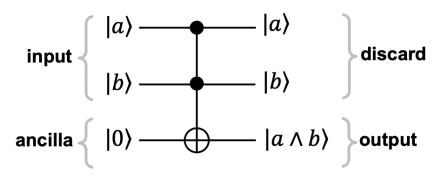
\includegraphics[width=0.5\linewidth]{Images/toffoli_classical.png}
        \caption{Using a Toffoli gate to simulate classical AND gate}
        \label{fig:toffoli_classical}
    \end{figure}
    Bits are represented as computational basis states in the natural way (bits $a,b \in \{0,1\}$ are represented by $\ket{a}$ and $\ket{b}$). To compute the AND of a and b, third ancilla qubit in state $\ket{0}$ is added and then a Toffoli gate is applied as shown in figure \ref{fig:toffoli_classical}. This causes the state of the ancilla qubit to become $\ket{a \land b}$. The first two qubits can be discarded, or just ignored for the rest of the computation. That's how an AND gate can be simulated.

    To simulate NOT gates, we can use the Pauli X gate.
    Finally, we can explicitly simulate a fan-out gate by adding an ancilla in state $\ket{0}$ and apply a CNOT gate, as shown in figure \ref{fig:CNOT_fanout}.
    \begin{figure}[ht]
        \centering
        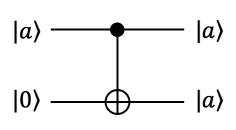
\includegraphics[width=0.3\linewidth]{Images/CNOT_fanout.png}
        \caption{Using a CNOT gate to simulate a classical fan-out gate}
        \label{fig:CNOT_fanout}
    \end{figure}
    Note that we defined quantum circuits to be in terms of 1-qubit and 2-qubit gates, but our simulation of classical circuits used 3-qubit gates: the Toffoli gate. We can remedy this by simulating each Toffoli gate by a series of 2-qubit gates. Let's  show how to do this. To start, we will make use of a $2\times 2$ unitary matrix with the property that if you square it you get Pauli X. Since X is essentially the NOT gate, this matrix is sometimes referred to as ``square root of NOT". Note that, in classical information, there is no square root of NOT, so the quantum square root of NOT can be regarded as a curiosity. Let's refer to this matrix as V. Henceforth, assumed that we have such a matrix V in hand. From this, we can define a controlled-V gate. Also, we can define a controlled-$V^{\dagger}$ gate. Now, consider the following circuit in figure \ref{fig:toffoli_2-qubit}, consisting of 2-qubit gates.
    \begin{figure}[ht]
        \centering
        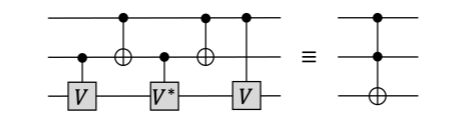
\includegraphics[width=0.75\linewidth]{Images/squarerootx.png}
        \caption{Simulating a Toffoli gate in terms of 2-qubit gates}
        \label{fig:toffoli_2-qubit}
    \end{figure}
    This computes Toffoli gate.
    we can work out the $ 8 \times 8$ matrix corresponding to each gate and then multiply the five matrices and see if the product is the matrix for the toffoli gate.

    A second approach is to verify that the circuits are equivalent in the case where the first two qubits are in computational basis states $\ket{00},\ket{01},\ket{10},\ket{11}$. 

Thinking about this way, we can gain some intuition about wy the circuit works. in the future if you need to design a quantum circuit to achieve something, such intuition can be helpful. 

Some classical algorithms make use of random number generators and we have not captured this in our definition of classical circuits. Say we allow our classical algorithms to access random bits, that are zero with probability $\frac{1}{2}$ and one with probability $\frac{1}{2}$. Can we simulate such random bits with quantum circuits? This is actually quite easy, since constructing a $\ket{+}$ state and measuring it yields a random bit. But this entails an intermediate measurement. Our quantum circuits will not look like ones we defined earlier, where all the measurements are at the end. Can we simulate random bits without the intermediate measurements? the answer is yes, by the following construction
\begin{figure}[ht]
    \centering
    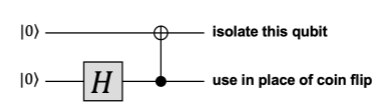
\includegraphics[width=0.5\linewidth]{Images/randbit_sim.png}
    \caption{Simulating random bits without using measurements}
    \label{fig:randbit_sim}
\end{figure}
Instead of measuring the qubit in the $\ket{+}$ state, we apply a CNOT gate to a target qubit (an ancilla) in the state $\ket{0}$. Then we ignore that ancilla qubit for the rest of the computation. The final probabilities when the circuits is measured at the end will be exactly the same as if a random bit had been inserted at that place in the computation.
\end{proof}
Using our decomposition of the Toffoli gate into 2-qubit gates and our results about simulating classical randomness, we can strengthen the above theorem to the following:
\begin{corollary}
    Any classical probabilistic circuit of size s can be simulated by a quantum circuit of size $\mathcal{O}(s)$, consisting of 1-qubit and 2-qubit gates.
\end{corollary}
\subsection{Fixed Point Number Representation and Classical Arithmetic operations}
Any integer $k \in [N]=\{0,1,\cdots,N-1\}$ where $N=2^n$ can be expressed as n n-bit string as
$k=k_{n-1}\cdots ,k_0$  with $k_i \in \{0,1\}$. This is called binary representation of integer k.
\[
k=\sum_{i \in [n]}k_i2^i
\]
The number k divided by $2^m \quad (0\leq m\leq n)$ (note that the decimal is shifted to be after $k_m$).
\[
a=\frac{k}{2^m}=\sum_{i\in [n]}k_i2^{i-m}=(k_{n-1}\cdots k_m.k_{m-1}\cdots k_0)\]
when m=n,
\[
a=\frac{k}{2^n}=\sum_{i\in [n]}=\sum_{i\in[n]}k_i2^{i-n}=0.k_{n-1}\cdots k_0
\]
 
$a=0.k_{n-1}\cdots k_0$ so that $k_i$ is the ith decimal of a in the binary representation. Note that here $0\leq a\leq 1$.
The number $(0.k_{n-1}\cdots k_i)$ is called n-bit fixed point representation of a. Therefore to represent a the additive precision $\epsilon$,
$n=\lceil\log_2(\epsilon)\rceil$ qubits are required. We may add one extra bit to indicate its sign.
 
Thus, we can perform classical arithmetic operations, such as $(x,y)\rightarrow x+y,(x,y)\rightarrow xy,x \rightarrow x^{\alpha}, x\rightarrow \cos\alpha $ etc.
using reversible quantum circuits. The number of ancilla qubits, and the number of elementary gates needed for implementing such circuits is $\mathcal{O}(poly(n))$.
Thus, quantum computer is theoretically as powerful as classical computers, there is a very significant overhead in implementing reversible classical circuits on quantum devices, both in terms of the number
of ancilla qubits and the circuit depth.


\section{Energy and computation}
Computational complexity theory studies the amount of time and space required to solve a computational problem. Another important computational resource is energy. In this section, we study the energy requirements for computational. Surprisingly, it turns out that computation, both classical and quantum, can in principle be done without expending any energy! Energy consumption in computation turns out to be deeply linked to the reversibility of computation. Consider a gate like the NAND gate, which takes an input two bits, and produces a single bit as output. This gate is intrinsically irreversible because, given the output of the gate, the input is not uniquely determined. For example, if the output of the NAND gate is 1, then the input could have been any one of 00, 01 or 10. On the other hand, the NOT gate is an example of a reversible logic gate because, given the output of the NOT gate, it is possible to infer what the input must have been.

Another way of understanding irreversibility is to think of it in terms of information erasure. if a logic gate is irreversible, then some of the information input to the gate is lost irretrievably when the gate opens -that is, some of the information has been erased by the gate. Conversely, in a reversible computation, no information is ever erased, because the input can always be recovered from the output. Thus, saying that a computation is reversible is equivalent to saying that no information is erased during the computation.

What is the connection between energy consumption and irreversibility in computation? Landaeur's principle provides the connection, stating that, in order to erase information, it is necessary to dissipate energy. More precisely, Landaeur's principle may be stated as follows:
\begin{definition}
    \textbf{Landaeur's principle (first form)}: Suppose a computer erases a single bit of information. The amount of energy dissipated into the environment is at least $k_BTln 2$, where $k_B$ is a universal constant known as Boltzmann's constant, and $T$ is the temperature of the environment of the computer.
\end{definition}

According to the laws of thermodynamics, Landaeur's principle can be given an alternative form stated not in terms of energy dissipation, but rather in terms of entropy.

\begin{definition}
    \textbf{Landaeur's principle (second form)}: Suppose a computer erases a single bit of information. The entropy of the environment increases by at least $k_b Tln 2$, where $k_b$ is Boltzmann's constant.
\end{definition}

Justifying Landaeur's principle is a problem of physics. If we accept Landaeur's principle as given, then it raises a number of interesting questions. First of all, Landaeur's principle only provides a lower bound on the amount of energy that must be dissipated to erase information. How close are existing computers to this lower bound? Not very, turns out to be the answer - computers circa the year 2000 dissipate roughly $500k_n Tln2$ in energy for each elementary logical operation.

Although existing computers are far from the limit set by Landaeur's principle, it is still an interesting problem of principle to understand how much the energy consumption can be reduced. Aside from the intrinsic interest of the problem, a practical reason for the interest follows from Moore's law: if computer power keeps increasing them the amount of energy dissipated must also increases unless the energy dissipated per operation drops at least as fast as the rate of increasing computing power.

If all computations could be done reversibly, then Landaeur's principle would imply no lower bound on the amount of energy dissipated by the computer, since no bits at all are erased during a reversible computation. Of course, it is possible that some other physical principle might require that energy dissipated during the computation: fortunately, this turns out not to be the case. But is it possible to perform universal computation without erasing any information? Physicists can cheat on this problem to see in advance that the answer to this question must be yes, because our present understanding of the laws of physics is that they are fundamentally reversible. That is, if we know the final state of a closed physical system, then the laws of physics allows us to work out the initial state of the system. If we believe that those laws are correct, then we must conclude that hidden in the irreversible logic gates like AND and OR, there must be some underlying reversible computation. But where is the hidden reversibility, and can we use it to construct manifestly reversible computers?

We will use two different techniques to give reversible circuit-based models capable of universal computation. The first model, a computer built entirely of billiard balls and mirrors, gives a beautiful concrete realization of the principles of reversible computation. The second model, based on a reversible logic gate known as the Toffoli gate, is a more abstract view of reversible computation. It is also possible to build reversible Turing machines that are universal for computation; however we won't study these here, since the reversible circuit models turns out to be much more useful for quantum computation.

\subsection{The billiard ball model of computation}
The basic idea of the billiard ball computer is illustrated in figure \ref{fig:billiardballmodel}. Billiard ball `inputs' enter the computer from the left hand side, bouncing off mirrors and each other, before exiting as `outputs' on the right hand side. The presence or absence of a billiard ball at a possible input side is used to indicate a logical 1 or a logical 0, respectively. The fascination thing about this model is that it is manifestly reversible, in so far its operation is based on the laws of classical mechanics. Furthermore, this model of computation turns out to be universal in the sense that it can be used to simulate an arbitrary computation in the standard circuit model of computation.
\begin{figure}[ht]
    \centering
    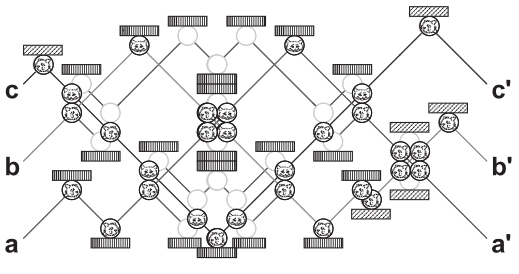
\includegraphics[width=1\linewidth]{Images/blliardballmodel.png}
    \caption{A simple billiard ball computer, with three input bits and three output bits, shown entering on the left and leaving on the right, respectively. The presence or absence of a billiard ball indicates a $1$ or a $0$, respectively. Empty circles illustrate potential paths due to collisions. This particular computer implements the Fredkin classical reversible logic gate, discussed in the text.}
    \label{fig:billiardballmodel}
\end{figure}
Of course, if a billiard ball computer were ever built it would be highly unstable. As any billiard player can attest, a billiard ball rolling frictionlessly over a smooth surface is easily knocked off course by small perturbations. The billiard ball model of computation depends on perfect operation, and the absence of external perturbations such as those caused by thermal noise. Periodic corrections can be performed, but information gained by doing this would have to be erased, requiring work to be performed. Expenditure of energy thus serves the purpose of reducing this susceptibility to noise, which is necessary for practical, real-world computational machine. For this purpose of this introduction we will ignore the effects of noise on the billiard ball computer, and concentrate on understanding the essential elements of reversible computation.

The billiard ball computer provides an elegant means for implementing a reversible universal logic gate known as the Fredkin gate. Indeed, the properties of the Fredkin gate provide an informative overview of the general principles of reversible logic gates and circuits. The Fredkin gate has three input bits and three output bits, which we refer to as $a,b,c$ and $a',b',c'$, respectively. The bit $c$ is a control bit, whose value is not changed but he action of the Fredkin gate, that is, $c'=c$. The reason $c$ is called the control bit is because it controls what happens to the other two bits, $a$ and $b$. If $c$ is set to $0$ then $a$ and $b$ are left alone, $a'=a$ and $b'=b$. If $c$ is set to 1, $a$ and $b$ are swapped, $a'=b$, $b'=a$. The explicit truth table for the Fredkin gate is shown in table \ref{fig:fredcircimple}. It is easy to see that the Fredkin gate is reversible, because given the output $a',b',c'$, we can determine the inputs $a,b,c$. In fact, to recover the original inputs $a,b$ and $c$ we need only apply another Fredkin gate to $a',b',c'$:
\begin{figure}[ht]
    \centering
    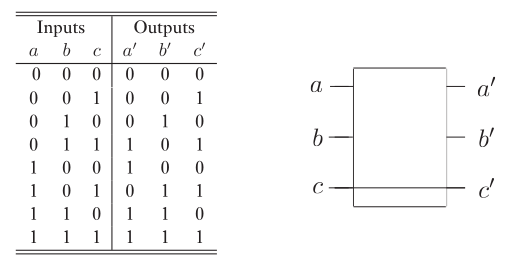
\includegraphics[width=1\linewidth]{Images/fredkingateandcircimpl.png}
    \caption{Fredkin gate truth table and circuit representation. The bits $a$ and $b$ are swapped if the control bit $c$ is set, and otherwise are left alone}
    \label{fig:fredcircimple}
\end{figure}
\begin{example}
    \textbf{(Fredkin gate is self-inverse)} Show that by applying two consecutive Fredkin gates gives the same outputs as inputs.
\end{example}
Examining the parts of the billiard balls in figure \ref{fig:billiardballmodel}, it is not difficult to verify that this billiard ball computer implements the Fredkin gate.

\begin{example}
    Verify that the billiard ball computer in figure \ref{fig:billiardballmodel} computes the Fredkin gate.
\end{example}

In addition to reversibility, the Fredkin gate also has the interesting property that the number of 1s is conserved between the input and output. In terms of the billiard ball computer, this corresponds to the number of billiard balls going into the Fredkin gate being equal to the number coming out. Thus, it is sometimes referred to as being a conservative reversible logic gate. Such reversibility and conservative properties are interesting to a physicist because they can be motivated by fundamental physical principles. The laws of Nature are reversible, with the possible exception of the measurement postulate of quantum mechanics. The conservative property can be through of as analogous to properties such as conservation of mass, or conservation of energy. indeed, the billiard ball model of computation the conservative property corresponds exactly to conservation of mass.

The Fredkin gate is not only reversible and conservative, it's a universal logic gate as well!!. Note that NAND and other classical gates (such as AND, OR, etc..) are not reversible gates! Thus, we need to convert the classical gates to reversible gates. Any irreversible classical gate $x \rightarrow f(x)$ can be converted to a reversible gate by adding an extra bit called the ``ancilla bit" and then applying the reversible gate. One of the ways is to store all the intermediate steps of the computation. On the quantum computer, storing all the intermediate steps is problematic because of waste of quantum resources as those qubits can then be never used again, and intermediate bits stored in some extra qubits are still entangled to the quantum state of interest. (If the environment interferes with the intermediate result, then the quantum state of interest also gets affected).

As illustrated in figure \ref{fig:fredimpdiff}, the Fredkin gate can be configured to simulate AND, NOT, CROSSOVER and FANOUT functions, and thus can be cascaded to simulate any classical circuit whatsoever.
\begin{figure}[ht]
    \centering
    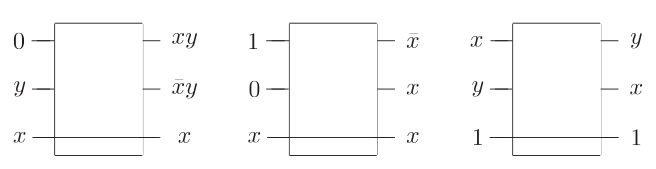
\includegraphics[width=0.5\linewidth]{Images/fredimplediff.png}
    \caption{Fredkin gate configured to perform the elementary gates AND (left), NOT(middle), and a primitive routing function, the CROSSOVER (right). The middle gate also serves to perform the FANOUT operation, since it produces two copies of $x$ at the output. Note that each of these configuration requires the use of extra `ancilla' bits prepared in standard states - for example, the input $0$ input on the first line of the AND gate - and in general the output contains `garbage' not needed for the remainder of the computation.}
    \label{fig:fredimpdiff}
\end{figure}
To simulate irreversible gates such as AND using the Fredkin gate, we made use of two ideas. First, we allowed the input of `ancilla' bits to the Fredkin gate, in specially prepared states, either 0 or 1. Second, the output of the Fredkin gate contained extraneous `garbage' not needed for the remainder of the computation. The ancilla and garbage bits are not directly important to the computation. Their importance lies in the fact that they make the computation reversible. Indeed the irreversibility of gates like the AND and OR may be viewed as a consequence of the ancilla and garbage bits being `hidden'. Summarizing, given any classical circuit computing a function $f(x)$, we can build a reversible circuit made entirely of Fredkin gates, which on input of $x$, together with some ancilla bits in a standard state $a$, computes $f(x)$, together with some extra `garbage' output, $g(x)$. Therefore, we represent the action of the computation as $(x,a)\rightarrow (f(x),g(x))$.

We now know how to compute function reversibly. Unfortunately, this computation produces unwanted garbage bits $g(x)$. With some modifications it turns out to be possible to perform the computation so that any garbage bits produced are in a standard state. This construction is crucial for quantum computation, because garbage bits whose values depends upon $x$ will in general destroy the interference properties crucial to quantum computation. To understand how this works it is convenient to assume that the NOT gate is available on our repertoire of reversible gates, so we may as well assume that the ancilla bits $a$ all start out as 0s, with NOT gate being added where necessary to turn the ancilla 0s into 1s. It will also be convenient to assume that the classical controlled-NOT gate is available, that is, the inputs $(c,t)$ are taken to $(c,t\oplus c)$, where $\oplus$ denotes addition modulo $2$. Notice that $t=0$ gives $(c,0)\rightarrow (c,c)$ , so the controlled-NOT can be though of as a reversible copying gate or FANOUT, which leaves no garbage bits at the output.

With the additional NOT gates appended at the beginning of the circuit, the action of the computation may be written as $(x,0)\rightarrow (f(x),g(x))$. We could also ad CNOT gates to the beginning of the circuit, in order to create a copy of $x$ which is not changed dugring the subsequeunt computation. With this modification, the circuit may be written as
\[
(x,0,0)\rightarrow (x,f(x),g(x))
\]
This is a very useful way of writing the action of the reversible circuit, because it allows an idea known as uncomputation to be used to get rid of the garbage bits, for a small cost in the running time of the computation. The idea is the following. Suppose we start with a four register computer in the state $
(x,0,0,y)$. The second register (also called ancilla qubits) is used to store the result of the computation, and the third register is used to provide workspace for the computation (also called working register aka garbage register - they are ancilla registers which can be freed after uncomputation), that is, the garbage bits $g(x)$. The use of the fourth register is described shortly, and we assume it starts in an arbitrary state $y$.

We begin as before, by applying a reversible circuit to compute $f$, resulting in the state $(x,f(x),g(x),y)$. From no deletion theorem, there is no generic unitary operator that can set a black-box state to $0$. We wish to set the working registers back to $0$ while keeping the input and output state. Next, we use CNOTs to add the result $f(x)$ bitwise to the fourth register, leaving the machine in the state $(x,f(x),g(x),y\oplus f(x))$. Note that here the CNOT gates only perform the classical XOR operation (or classical copying operation if $y=0$ in the computational basis) and thus does not violate the \textit{No-Cloning Theorem}. Note that all the steps used to compute $f(x)$ were reversible $(U_f^{\dagger}=U_f^{-1})$ and did not affect the fourth register, so by applying the reverse of the circuit used to compute $f$ we come to the state $(x,0,0,y\oplus f(x))$. We can then apply a SWAP operation on the working registers and the ancilla registers to obtain $(x,0,0,y\oplus f(x))\rightarrow (x,y\oplus f(x),0,0)$. Thus, note that the working registers (aka garbage registers) are set to $0$ and are no longer entangled to the input or output register and can be reused for other purposes. This is called \textbf{Uncomputation}. Thus, after the uncomputation step the second and thrid regsiters as shown are unchanged before and after the application of the circuit, though they are changed during the intermediate steps. Typically, we omit the ancilla $0s$ from the description of the function evaluation, and just write the action of the circuit as
\[
(x,y)\rightarrow (x,y\oplus f(x))
\]
allowing us to simplify notation and focus on the essence of Quantum Algorithm. In general we refer to this modified circuit computing $f$ as the reversible circuit computing $f$, even though in principle there are many other reversible circuits which could be used to compute $f$. The reversible gate is thus defined as $(x,y)\rightarrow (x,f(x)\oplus y)$. Thus, in particular we have $(x,0)\rightarrow (x,f(x))$ where $0$ are the ancilla qubits required. Note that we have not considered the working register here because they can be freed after the computation via uncomputation and thus can be further used in the computation.

What resource overhead is involved in doing reversible computation? To analyze this question, we need to count the number of extra ancilla bits needed in a reversible circuit, and compare the gate counts with classical models. It ought to be clear that the number of gates in a reversible circuit is same as in an irreversible circuit to within the constant factor which represents the number of Fredkin gates needed to simulate a single element of the irreversible circuit, and an additional factor of two for uncomptation with an overhead for the extra CNOT operation used in reversible computation which is linear in the number of bits involved in the circuit. Similarly, the number of ancilla bits required scales at most linearly with the number of gates in the irreversible circuit, since each element in the irreversible circuit can be simulated using a constant number of ancilla bits. As a result, natural complexity classes such as $P$ and $NP$ are the same not matter whether a reversible or irreversible model of computation is used.

Thus, the technique of uncomutation, if the map $x\rightarrow f(x)$ can be efficiently implemented on a classical computer, then we can implement the map efficiently on a quantum computer as well. All reversible single-bit and two-bit classical gates can be implemented using single-bit and two-bit quantum gates. Thus, the reversible map can be made into a unitary operation as
\[
U_f\ket{x,y}\rightarrow \ket{x,y\oplus f(x)}
\]
This, proves that quantum computers are at least as powerful as classical computers. $U_f$ can be applied to any superposition of the states in the computational basis. Thus, the quantum computer can perform the computation on all possible inputs simultaneously.
\[
U_f:\frac{1}{\sqrt{2^n}}\sum_{x\in\{0,1\}^n} \ket{x,0}\rightarrow \frac{1}{\sqrt{2^n}}\sum_{x\in\{0,1\}^n}\ket{x,f(x)}
\]

This does not necessarily mean that we can efficiently implement the map $\ket{x}\rightarrow \ket{f(x0}$. If $f$ is a bijection, and we have access to the inverse of the reversible circuit for computing $f^{-1}$ then we may use the technique of uncomputation to implement such a map.

\begin{example}
    \textbf{(Reversible half-adder)} Construct a reversible circuit, when two bits $x$ and $y$ are input, outputs $(x,y,c,x\oplus y)$, where $c$ is the carry bit when $x$ and $y$ are added.
\end{example}

The Fredkin gate and its implementation using the billiard ball computer offers a beautiful paradigm for reversible computation. There is another reversible logic gate, the Toffoli gate, which is also universal for classical computation. While the Toffoli gate does not have qubit the same elegant physical simplicity as the billiard ball implementation of the Fredkin gate, it will be more useful in the study of quantum computation. For convenience, we review its properties here.
\begin{figure}[ht]
    \centering
    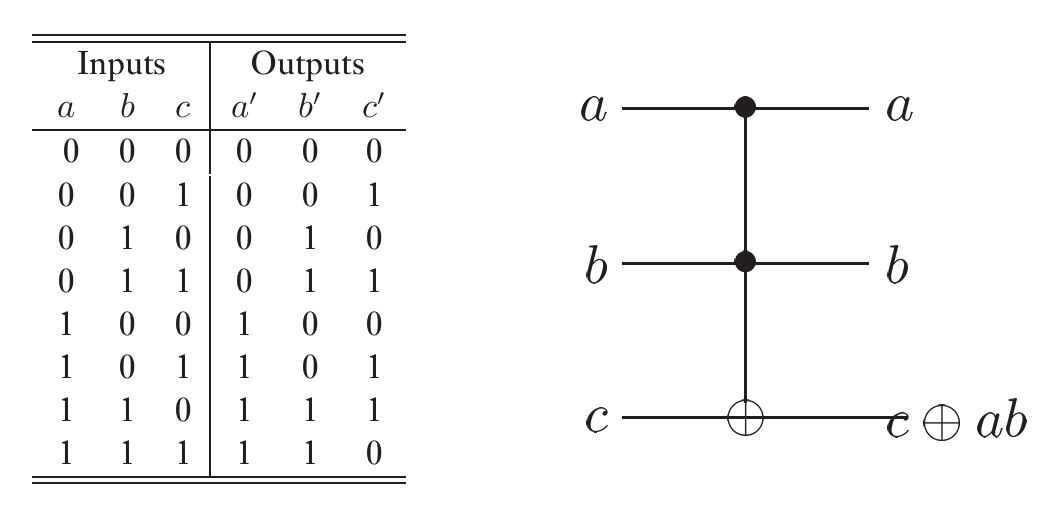
\includegraphics[width=0.75\linewidth]{Images/toffolitru.png}
    \caption{Truth table and circuit representation for the Toffoli Gate}
    \label{fig:toffolitruth}
\end{figure}
The Toffoli gate has three input bits, $a,b$ and $c$. $a$ and $b$ are known as the first and second control bits, where $c$ is the target bit. The gate leaves both control bits unchanged, flips the target bit if both control bits are set, and otherwise leaves the target bit alone. The truth table and the circuit representation for the Toffoli gate are as shown in the figure \ref{fig:toffolitruth}.
\begin{figure}[ht]
    \centering
    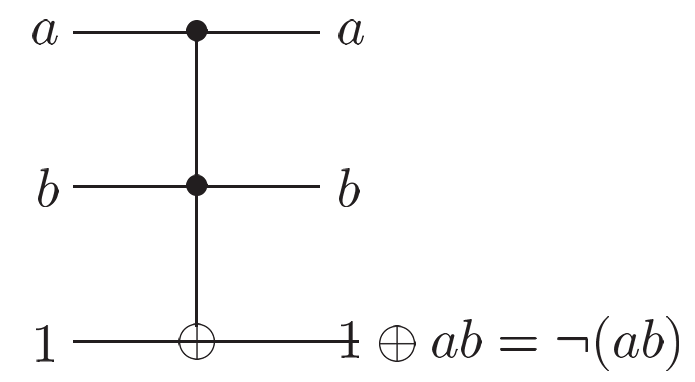
\includegraphics[width=0.5\linewidth]{Images/NANDToffoli.png}
    \caption{Implementing NAND gate using a Toffoli gate. The top two qubits represnt the input to the NAND, while the third bit is prepared in the state 1, sometimes known as the ancilla state. The output from the NAND is in the third bit.}
    \label{fig:NANDToff}
\end{figure}
How can the Toffoli gate be used to do universal computation? Suppose we wish to NAND the bits $a$ and $b$. To do this using the Toffoli gate, we input $a$ and $b$ as control bits, and send in an ancilla bit set to $1$ as the target bit, as shown in figure \ref{fig:NANDToff}. The NAND of $a$ and $b$ is output as the target bit. As expected from our study of the Fredkin gate, the Toffoli gate simulation of a NAND requires the use of a special ancilla input, and some of the outputs from the simulation are garbage bits.
\begin{figure}[ht]
    \centering
    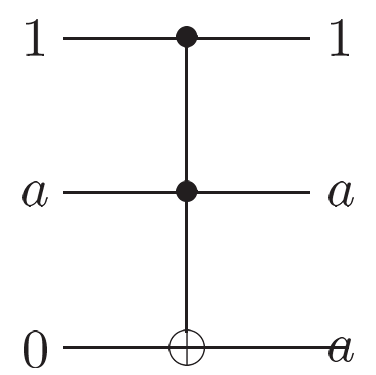
\includegraphics[width=0.25\linewidth]{Images/FANOUT.png}
    \caption{FANOUT with the Toffoli gate, with the second bit being the input to the FANOUT, and the other two bits standard ancilla bits. he output from the FANOUT appears on the second and the third bits.}
    \label{fig:FANOUTToff}
\end{figure}
The Toffoli gate can also be used to implement the FANOUT operation by inputting an ancilla $1$ to the first control bit, and $a$ to the second control bit, producing the output $1,a,a$. This is illustrated in figure \ref{fig:FANOUTToff}. Recalling that NAND and FANOUT are together universal for computation, we see that na arbitrary circuit can be efficiently simulation using a reversible circuit consisting only of Toffoli gates and ancilla bits, and that useful additional techniques such as uncomputation may be achieved using the same methods as were employed with the Fredkin gate.

Our interest in reversible computation was motivated by our desire to understand the energy requirements for computation. It is clear that the noise-ree billiard ball model of computation requires no energy for its operation; what about models based upon the Toffoli gate? This can only be determined by examining specific models for the computation of the Toffoli gate. It turns out that, indeed, the Toffoli gate can be implemented in a manner which does not require expenditure of energy.

There is a significant caveat attached to the idea that computation can be done without the expenditure of energy. As we noted earlier, the billiard ball model of computation is highly sensitive to noise, and this is true of many other models of reversible computation. To nullify the effects of noise, some form of error-correction needs to be done. Such error-correction typically involves the performance of measurements on the system to determine whether the system is behaving as expected or if an error has occurred. Because the computer's memory is finite, the bits used to store the measurement results utilized in error-correction must eventually be erased to make way for new measurement results. According to Landaeur's principle, this erasure carries an associated energy cost that must be accounted for when tallying the total energy of the computation. We analyze the energy cost associated with error correction in more detail in later chapters.

What can we conclude from our study of reversible computation? There are three key ideas. First, reversibility stems from keeping track of every bit of information; irreversibility occurs only when information is lost or erased. Second, by doing computation reversibly, we obviate the need for energy expenditure during computation. All computation can be done efficiently, without production of garbage bits whose value depends upon the input to the computation. That is, if there is an irreversible circuit computation a function $f$, then there is an efficient simulation of this circuit by a reversible circuit with the action $(x,y)\rightarrow (x,y\oplus f(x))$.

What are the implication of these result for physics, computer science, and for quantum computation and quantum information? From the point of view of a physicist or hardware engineer worried about head dissipation, the good news is that, in principle, it is possible to make computation dissipation -free by making it reversible, although in practice energy dissipation is required for system stability and immunity from noise. At an ever more fundamental level, the ideas leading to reversible computation also lead to the resolution of a century-old problem in the foundations of physics, the famous problem of Maxwell's demon. From the point of view of a computer scientist, reversible computation validates the use of irreversible models of computation such as the Turing Machine (since using them or not gives polynomially equivalent models). Moreover, since the physical world is fundamentally reversible, one can argue that complexity classes based upon reversible models of computation are more natural than complexity classes based upon irreversible models of computation. From the point of view of quantum computation and quantum information, reversible computation is enormously important. To harness the full power of quantum computation, any classical subroutines in a quantum computation must be performed reversibly and without the production of garbage bits depending on the classical input.

\begin{example}
    \textbf{(From Fredkin to Toffoli and back again)}
    What is the smallest number of Fredkin gates needed to simulate a Toffoli gate? What is the smallest number of Toffoli gates needed to simulate a Fredkin gate?
\end{example}


\begin{importantnote}
    \textbf{Maxwell's Demon}\\
    The laws of thermodynamics govern the amount of work that can be performed by a physical system at thermodynamic equilibrium. One of these laws, the second law of thermodynamics, states that the entropy in a closed system can never decrease. In 1871, James Clerk maxwell proposed the existence of a machine that apparently violated this law. He envisioned a miniature little `demon', like that shown in the figure below, which could reduce the entropy of a gas cylinder initially at equilibrium by individually separating the fast and slow molecules into the two halves of the cylinder. This demon would sit at a little door in the middle partition. When a fast molecule approaches from the left side the demon opens a door between the partitions, allowing the molecule through, and then closes the door. By doing this many times the total entropy of the cylinder can be decreased, in apparent violation or thermodynamics.

    The resolution of the Maxwell's demon paradox lies in the fact that the demon must perform measurements on the molecules moving between the partitions, in order to determine their velocities. The result of this measurement must be stored in demon's memory. Because any memory is finite, the demon must eventually begin erasing information from its memory, in order to have space for new measurement results. By Landauer's principle, this act of erasing information increase the total entropy of the combined system - demon, gas cylinder, and their environments. In fact, a complete analysis shows that Landauer's principle implies that the entropy of the combined system is increased at least as much by this act of erasing information as the entropy of the combined system is decreased by the actions of the demon, thus ensuring that the second law of thermodynamics is obeyed.
\end{importantnote}
\section{Efficient Implementation}
In order to implement Shor's algorithm, it is necessary to efficiently perform some of the arithmetic operations described above (modular exponentiation, in particular) with a quantum computer. Intuitively this seems like it should not be a problem, given that there is an efficient way to implement these operations classically. But does an efficient classical implementation necessarily imply the existence of an efficient quantum implementation? The fact that classical algorithms can use non-unitary operations such as ANDs and ORs, while quantum computers are restricted to unitary operations, makes this question non-trivial to answer.

Before we address the question of whether efficient classical algorithms for arithmetic problems (or any other type of computational problem) imply efficient quantum algorithms for these problems, we need to briefly discuss the notion of quantum circuit complexity. What does it mean to have an efficient quantum algorithm for some task?

Our answer to this question will be similar to the classical case. In order to completely specify a quantum algorithm, it is necessary to give a construct that produces a quantum circuit solving the problem at hand for any given input size. Also, as in the classical case, one assume the quantum circuit is composed entirely of quantum gates acting on small number of qubits-in analogy to the classical case,  one may require that all gates in the quantum circuit act on just one or two qubits. Again, to be considered efficient, one usually  requires that the number of gates is polynomially related to the number of input qubits.

There is, however, a crucial difference between the classical and quantum cases. Whereas there are a finite number of classical one and two bit operations, and it is well known that AND and NOT operations (for instance) are sufficient to generate any such operation, there are infinitely many one and two qubit operations. Although there are interesting technical aspects of this issue, such as the degree to which a finite number of quantum gates can approximate arbitrary gates, we will essentially sweep the issue under the rug by saying that arbitrary one and two qubit gates are allowed in our circuits.

By the way, it will be very helpful to use Toffoli gates to construct quantum circuits for various tasks. Recall that a Toffoli gate performs the transformation
\[
T\ket{a}\ket{b}\ket{c}=\ket{a}\ket{b}\ket{c \oplus (a \land b)}
\]
for $a,b,c\in\{0,1\}$. A Toffoli gate can be decomposed into one-an two-qubit quantum gates as follows:
\begin{figure}[ht]
    \centering
    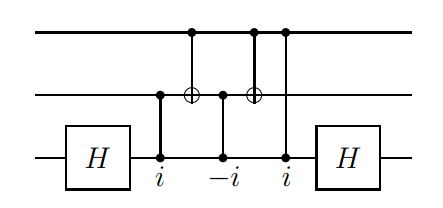
\includegraphics[width=0.5\linewidth]{Images/toffolidecompose.png}
\end{figure}
A careful check of the 8 standard basis states show that the circuit implements a Toffoli gate as claimed.

Now let us return to the question of whether an arbitrary efficient classical algorithm can be converted to an efficient quantum algorithm. Suppose that we have some classical Boolean circuit. For sake of example, suppose it performs modular additions as suggested in the following diagram.
\begin{figure}[ht]
    \centering
    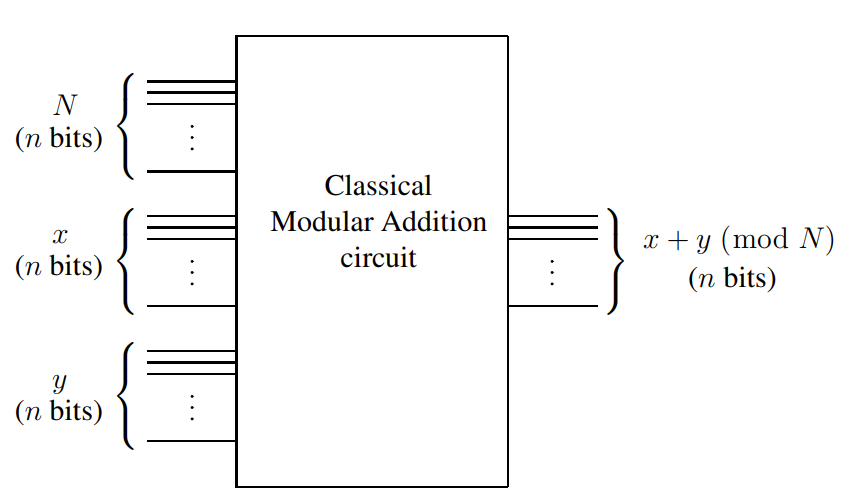
\includegraphics[width=0.5\linewidth]{Images/modularadditionclassical.png}
\end{figure}
Obviously, such a circuit is non-unitary-the number of input and output qubits do not even agree. If we are to somehow transform this circuit into a valid quantum circuit, it will have to correspond to a unitary transformation.

Based on our previous discussions concerning black-box transformations, we might hope to implement this operation unitarily as follows:
\begin{figure}[ht]
    \centering
    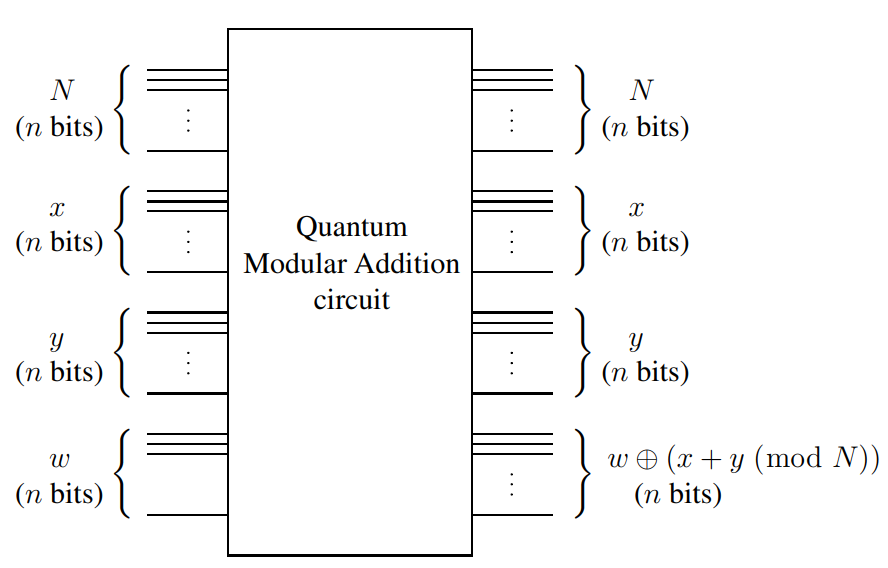
\includegraphics[width=0.5\linewidth]{Images/quantummodularaddition.png}
\end{figure}
This is a special type of unitary transformation, because it always maps classical states to classical states, therefore giving rise to a permutation matrix. We will show how to implement such transformations using only gates that map classical states to classical states, so none of what we are discussing right now needs to be thought of as inherently quantum. Usually when we are talking about quantum gates and circuits that always map classical states to classical states, we refer to them as reversible gates or circuits. In other words, a reversible gate is a special type of quantum gate that maps classical states to classical states, or equivalently gives rise to a permutation matrix.

Now let us see how we can transform the original classical circuit into such a circuit, obeying the constraint that only reversible gates are used inside the circuit. We do not want to have to reinvent the wheel, so to speak, so we can begin by trying to imply replace the gates of the classical circuit with reversible gates. The Toffoli gates will be handy for doing this.

\textbf{AND gate}. We can simulate AND gate using a toffoli gate as follows:\\
\begin{figure}[ht]
    \centering
    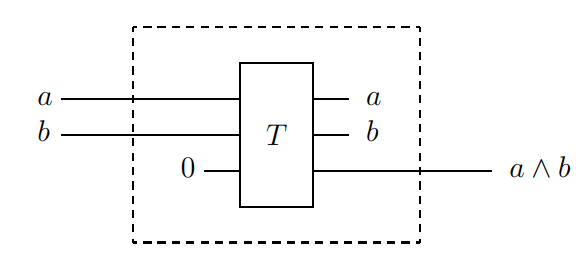
\includegraphics[width=0.5\linewidth]{Images/simulateand.png}
\end{figure}
\textbf{NOT gate} This is already unitary, so nothing needs to be done.

\textbf{OR gate} These can be replaced by an AND gate and three NOT gates using DeMorgan's Laws.

\textbf{FANOUT} We often do not even think of this as an operation, but we could have fanout in a classical Boolean circuit, and this needs to be explicitly implemented in a quantum circuit. Note that this does not mean replicating the quantum state of a qubit - it means replicating the classical state. here is how this operation can be simulated using a Toffoli gate:
\begin{figure}[ht]
    \centering
    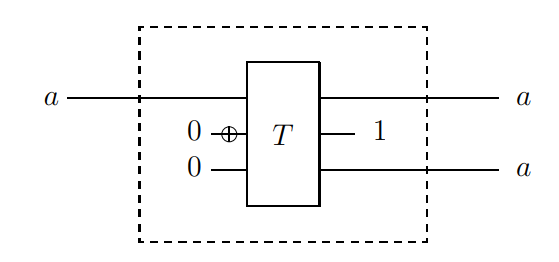
\includegraphics[width=0.5\linewidth]{Images/fanoutimg.png}
\end{figure}

Of course it would have been just as easy to input a 1 into the second input of the Toffoli fate rather than performing a NOT operation on a 0. I've only written it like this because it will be convenient later to have all of the auxiliary inputs start in the 0 state.

Now, we can simply go through the original circuit and replace each of the AND, OR, NOT, and FANOUT operations with reversible gates as just described,. if we started with a general circuit $C$ computing a function $f:\{0,1\}^n\rightarrow\{0,1\}^m$ as follows:
\begin{figure}[ht]
    \centering
    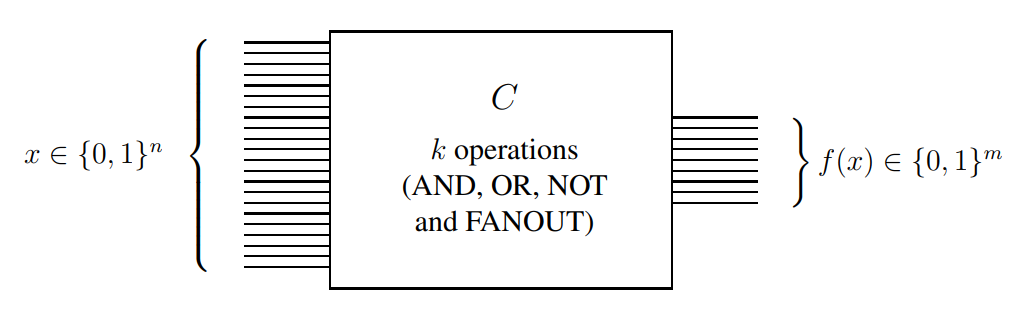
\includegraphics[width=0.5\linewidth]{Images/simulateclassical.png}
\end{figure}
Then we would end up with a reversible circuit $R$ as follows.
\begin{figure}[ht]
    \centering
    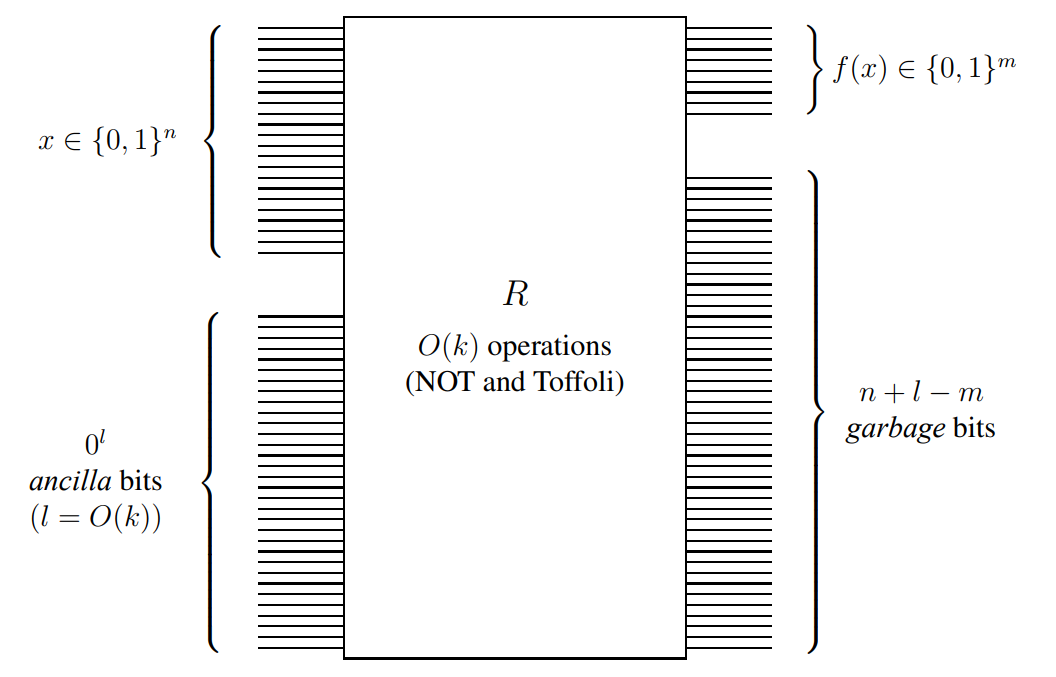
\includegraphics[width=0.75\linewidth]{Images/reversiblecomputecirc.png}
\end{figure}

The auxiliary bits needed for the AND and FANOUT simulations in this circuit are sometime called ancilla bits. The bits labeled garbage are the extra bits that resulted from the simulations (that were left inside the dashed boxes in the above pictures).

The circuit above is not quite what we want, because the garbage bits are undesirable - we have no control over them, and they would cause problems in many quantum computations. however, we almost have what we are after. by taking advantage of the fact that NOT gate and Toffoli gate are their own inverses (because they are unitary as well as Hermitian), we can simply take a ``mirror image" of $R$ to get $R^{-1}$, which simply undoes the computation of $R$. Combining $R,R^{-1}$, and a collection of controlled-NOT gates as described in figure essentially gives us what we are looking for. The only difference between this circuit and our initial aim is the existence of ancilla bits. (It should be noted that commonly when people use the term ``ancilla", they often expect that such bits are returned to their initial 0 state as in the circuit in Figure 1.) These bits will not have any adverse effects, and often we do not even explicitly mention them.

So, in summary, if you have a classical Boolean circuit $C$ for computing some function
\[
f:\{0,1\}^n \rightarrow \{0,1\}^m
\]
then the procedure above will transform a description of this circuit into a description of a quantum circuit $S_C$ composed only of Toffoli gates, NOT gates and controlled-NOT gates that satisfies
\[
S_C\ket{x}\ket{y}\ket{0^l}=\ket{x}\ket{y \oplus f(x)}\ket{0^l}
\]
\begin{figure}
    \centering
    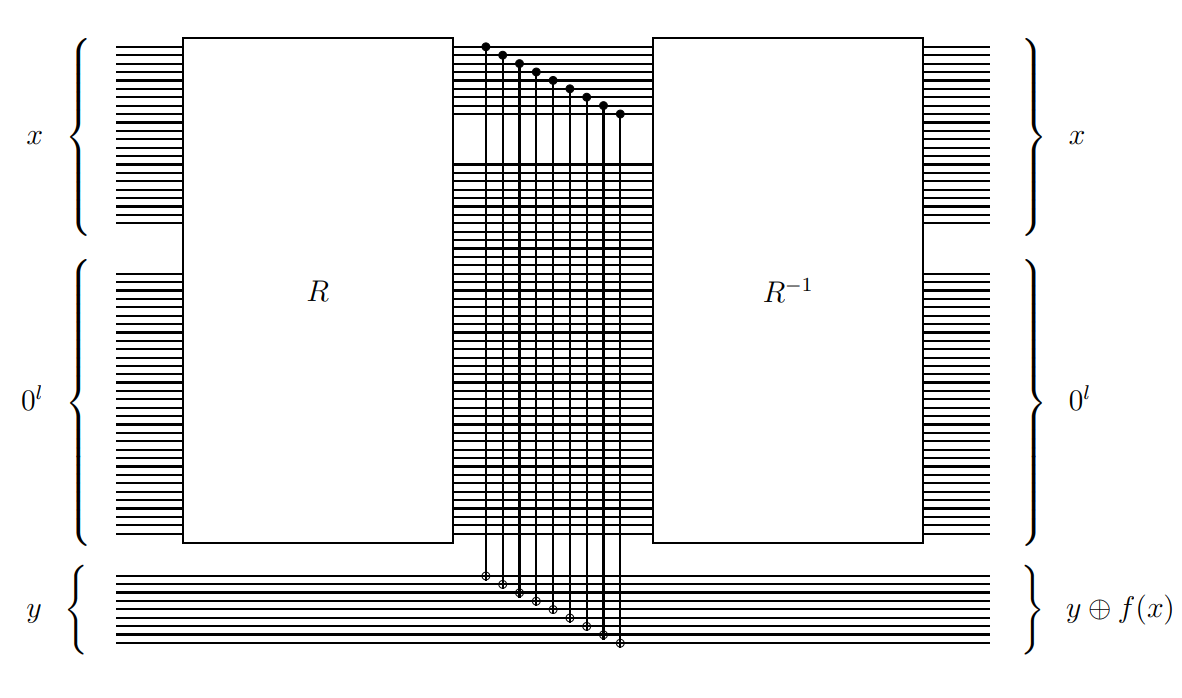
\includegraphics[width=0.75\linewidth]{Images/quantumreversiblecirc.png}
    \caption{The final reversible circuit $S_C$ implementing the transformation we are after}
    \label{fig:Sccirc}
\end{figure}
The number of ancilla qubits $l$ and the total number of gates in $S_C$ is linear in the number of operations in the original circuit $C$. The presence of ancilla qubits will have no effect on any algorithm that uses the circuit $S_C$, and in fact they could be re-used to perform some other transformation after $S_C$ is performed. For this reason, we will usually say that $S_C$ performs the transformation
\[
S_C\ket{x}\ket{y}=\ket{x}\ket{y \oplus f(x)}
\]
leaving it implicit that some number of ancilla qubits may have been used to implement $S_C$.

\subsection{Reversible Implementation of invertible functions}
Finally, suppose that you have a function of the form
\[
f:\{0,1\}^n\rightarrow \{0,1\}^n
\]
that itself is invertible (one-to-one and onto), and suppose that $f$ is efficiently computed by some Boolean circuit $C$. We already know that it is possible to build a reversible $S_C$ that performs the transformation
\[
S_C\ket{x}\ket{y}=\ket{x}\ket{y\oplus f(x)}
\]
for all $x,y \in\{0,1\}^n$ (possibly using some number of ancilla bits). Is it possible to go further and build a reversible circuit $Q$, possibly using some ancilla bits, that efficiently performs the transformation
\[
Q\ket{x}=\ket{f(x)}
\]
for all $x\in\{0,1\}^n$? because $f$ is assumed to be invertible, the transformation to be performed by $Q$ is indeed reversible, so in principle it is possible to build $Q$. The question, however, is about efficiency.

Without any further assumption it is not known how to construct $Q$ given only $C$. However, if in addition we have a Boolean circuit $D$ that efficiently computes $f^{-1}$, then $Q$ can be construct that efficiently performs the required transformation as follows:
\begin{figure}[ht]
    \centering
    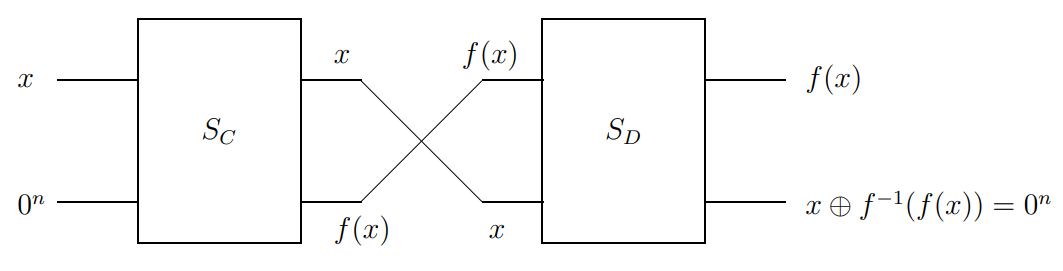
\includegraphics[width=0.75\linewidth]{Images/invertiblefunccirc.png}
\end{figure}
(In order to simplify the picture, each ``wire" represents n bits and the ancilla bits needed by the circuits $S_C$ and $S_D$ have not been shown explicitly.
We know that any classical Boolean circuit can be converted to a reversible (therefore unitary) circuit that efficiently implements the function computed by the original
circuit. For example, if the original Boolean circuit computes the function
\[
    f:\{0,1\}^n \rightarrow \{0,1\}^m
\]
then the reversible circuit efficiently implements the transformation
\[
    U_f:\ket{x}\ket{y} \rightarrow \ket{x}\ket{y\oplus f(x)}
\]
for all $x \in \{0,1\}^n$ and $y \in \{0,1\}^n$, possibly using some ancilla qubits that we do not
mention explicitly. Moreover, if 
\[
    f:\{0,1\}^n\rightarrow \{0,1\}^n 
\]
is invertible and we have a Boolean circuit for efficiently computing both $f$ and $f^{-1}$, then we can construct an efficient reversible circuit that performs the transformation
\[
P_f\ket{x}=\ket{f(x)}
\]
for all $x \in \{0,1\}^n$.
\section{Quantum Implementation of Classical Arithmetics operations}

Any sequence of quantum transforms effects a unitary transformation $U$ on the quantum systems. As long as no measurements are made, the initial quantum state of the system prior to a computation can be recovered from the final quantum state $\ket{\psi}$ by running $U^{-1}=U^{\dagger}$ on $\ket{\psi}$. Thus, any quantum computation is reversible prior to measurement in the sense that the input can always be computed from the output.

In contrast, classical computations are not in general reversible: it is noy usually possible to compute the input from the output. For example, while the classical NOT operation is reversible, the AND, OR, and NAND are not. Every classical computation does, however, have a classical reversible analog that takes only slightly more computational resources. We now show how to make basic Boolean gates reversible. Then show how to make entire Boolean circuits reversible in a resource efficient way, considering space, the number of qubits required, and the number of primitive gates. This construction of efficient classical reversible versions of arbitrary Boolean circuits easily generalizes to a construction of quantum circuits that efficiently implement general classical circuits.

Any classical reversible computation with $n$ input and $n$ output bits simply permutes the $N=2^n$ bit strings. Thus, for any such classical reversible computation there is a permutation $\pi:Z_N \rightarrow Z_N$ sending an input bit string to its output bit string. This permutation can be used to define a quantum transformation.

\[
U_{\pi}:\sum_{x=0}^{N-1}a_x\ket{x}\rightarrow \sum_{x=0\ket{\pi(x)}}
\]
that behaves on the standard basis vectors, viewed as classical bit strings, exactly as $\pi$ did. The transformation $U_{\pi}$ is unitary, since it simply reorders the standard basis elements.

Any classical computation on $n$ input and $m$ output bits defines function
\[
f:Z_N\rightarrow Z_M
\]
mapping the $N=2^n$ input bit strings to the $M=2^m$ output bit strings. Such a function can be extended in a canonical way to a reversible function $\pi_f$ acting on $n+m$ bits partitioned into two registers, the $n$-bit input register and the $m$-bit output register:
\[
\pi_f:Z_L\rightarrow Z_L
\]
\[
(x,y)\rightarrow \ket{(x,y\oplus f(x))}
\]
where $\oplus$ denotes the bitwise exclusive-OR. The function $\pi_f$ acts on the $L=2^{n+m}$ bit strings, each made up of an $n$-bit string $x$ and an $m$-bit string $y$. For $y=0$, the function $pi$ acts like $f$, except that the output appears in the output register and the input register retains the input. There are many other ways of making a classical computation reversible, and for a particular classical computation, there may be a reversible version that requires fewer bits, but this construction always works.

Since $\pi_f$ is reversible, there is a corresponding unitary transformation $U_f:\ket{x,y}\rightarrow \ket{x,y\oplus f(x)}$. Graphically the transformation $U_f$ is depicted as \ref{oracle}.

We have already shown how to implement any unitary operation in terms of simple gates. For most unitary transformations, that implementation is highly inefficient. while most unitary operators do not have an efficient implementation, $U_f$ has an efficient implementation as long as there is a classical circuit that computes $f$ efficiently. The method for constructing an efficient implementation of $U_f$ from an efficient classical circuit for $f$ has two parts. The first part constructs an efficient reversible classical circuit that computes $f$. The second part substitutes quantum gates for each of the reversible gates that make up the reversible classical circuit. We thus define reversible Boolean logic gates and convert the easy second part of the construction. We then explain the involved construction of an efficient reversible classical circuit for any efficient classical circuit.

\subsection{Reversible and Quantum versions of simple classical gates}
This section describes reversible versions of the Boolean logic gates NOT, XOR, AND, and NAND. Quantum versions of these gates act like the reversible gates on elements of the standard basis. Their action on other input states is prescribed by the linearity of quantum operations; the action of a gate on a superposition is the linear combination of the action of the gate on the standard basis elements making up the superposition. In this way, the behavior of a reversible gate fully defines the behavior of its quantum analog, and vice versa. The tight connection between the two allows us to use the same notation for both the gates with the understanding that the quantum gates can be applied to arbitrary superpositions, whereas the classical reversible gates are applied to bit strings that correspond to the standard basis elements.

Let $b_1$ and $b_0$ be two binary variables, variables taking on only values $0$ or $1$. We define the following quantum gates:

\subsubsection{NOT}
The NOT gate is already reversible. We will use $X$ to refer to both the classical reversible gate and the single-qubit operator $X=\ket{0}\bra{1}+\ket{1}\bra{0}$, which performs a classical NOT operation on classical bits encoded as the standard basis elements.

\subsubsection{XOR}
The controlled negation performed by the CNOT gate amounts to an $XOR$ operation on its input values. It retains the value of the first bit $b_1$, and replaces the value of the bit $b_0$ with the XOR of the two values.

The quantum version behaves like the reversible version on the standard basis vectors, and its behavior on all other states can be deduced from the linearity of the operator. 

\subsubsection{AND}
It is impossible to perform a reversible AND operation with only two bits. The three-bit controlled-controlled-NOT gate, or Toffoli gate, can be used to perform a reversible AND operation.
\[
CCNOT\ket{b_1b_0,0}=\ket{b_1b_0,b_1\land b_0}
\]
where $\land$ is notation for the classical AND of the two bit values.

The Toffoli gate is defined for all input: when the value of the third bit is $1$,
\[
CCNOT\ket{b_1b_0,1}=\ket{b_1b_0,1\oplus b_1\land b_0}
\]
By varying the values of input bits, the Toffoli gate $T$ can be used to construct a complete set of Boolean connectives, not just the classical AND. Thus, any combinatorial circuit can be constructed from Toffoli gates alone. The Toffoli gate computes NOT, AND, XOR, and NAND in the following way:
\[
CCNOT\ket{1,1,x}=\ket{1,1,\neg x}
\]
\[
CCNOT\ket{x,y,0}=\ket{x,y,x\land y}
\]
\[
CCNOT\ket{1,x,y}=\ket{1,x,x\oplus y}
\]
\[
CCNOT\ket{x,y,1}=\ket{x,y,\neg(x\land y)}
\]
where $\neg$ indicates the classical NOT acting on the bit value.

An alternative to the Toffoli gate, the Fredkin gate $F$, acts as a controlled swap. The Fredkin gate $F$, like the Toffoli gate, can implement a complete set of classical Boolean operators:
\[
F\ket{x,0,1}=\ket{x,x,\neg x}
\]
\[
F\ket{x,y,1}=\ket{x,y\lor x,y\lor \neg x}
\]
\[
F\ket{x,0,y}=\ket{x,y\land x,y \lor \neg x}
\]
where $\lor$ is the notation for the classical OR of the two bit values.

Because a complete set of classical Boolean connectives can be implemented using just the Toffoli gate, or the Fredkin gate $F$, these gates can be combined to realize arbitrary Boolean circuits. We now describe the explicit implemntation of certain classical functions. As the equations for the Toffoli gate illustrate, the operations CNOT and $X$ can be implemented by Toffoli gate with the addition of one or two bits permanently set to $1$. For clarity, we use CNOT and $X$ gates in our construction, but all constructions can be done using only Toffoli gates, since we can replace all uses of CNOT and $X$ with Toffoli gates that have additional input bits with their input value set appropriately. For example, the circuit shown in figure \ref{fig:onebitadd} implements a one-bit full adder using Toffoli and controlled-NOT gates, where $x$ and $y$ are the data bits, $s$ is their sum (modulo $2$), $c$ is the incoming carry bit, and $c'$ is the new carry bit. Several one-bit adders can be strung together to achieve full $n$-bit addition.
\begin{figure}
    \centering
    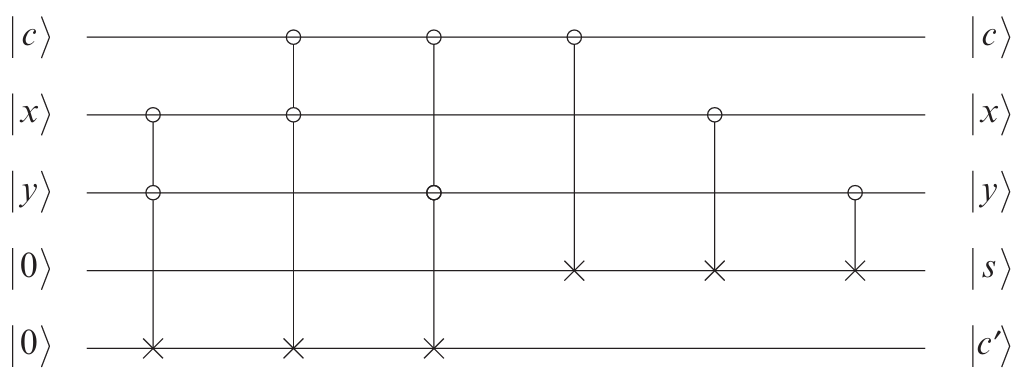
\includegraphics[width=0.5\linewidth]{Images/one-bitadd.png}
    \caption{One-bit Full adder}
    \label{fig:onebitadd}
\end{figure}
\section{Reversible implementation of Classical Circuits}
This section develops systematic way to turn arbitrary classical Boolean circuits into reversible classical circuits of comparable computational efficiency in terms of the number of bits and the number of gates. The resulting reversible circuits are composed entirely of Toffoli and negation gates. A quantum circuit with the same efficiency as the classical reversible circuit is obtained by the trivial substitution of quantum Toffoli and $X$ gates for classical Toffoli and negation gates. Thus, as soon as we have an efficient version of a computation in terms of Toffoli gates, we immediately know how to obtain a quantum implementation of the same efficiency.

\subsection{A Naive reversible Implementation}
Rather than start with arbitrary Boolean circuits, we consider a classical machine that consists if a register of bits and a processing unit. The processing unit performs simple Boolean operations or gates on one or two of the bits in the register at a time and stores the result in one of the register's bits. We assume that, for a given size input, the sequence of operations and their order of execution are fixed and do not depend on the input data or on other external control. In analogy, with quantum circuits, we draw bits of the register as horizontal lines. A simple program (for four-bit conjunction) or this kind of machine is depicted in figure \ref{fig:4bitconj}.
\begin{figure}
    \centering
    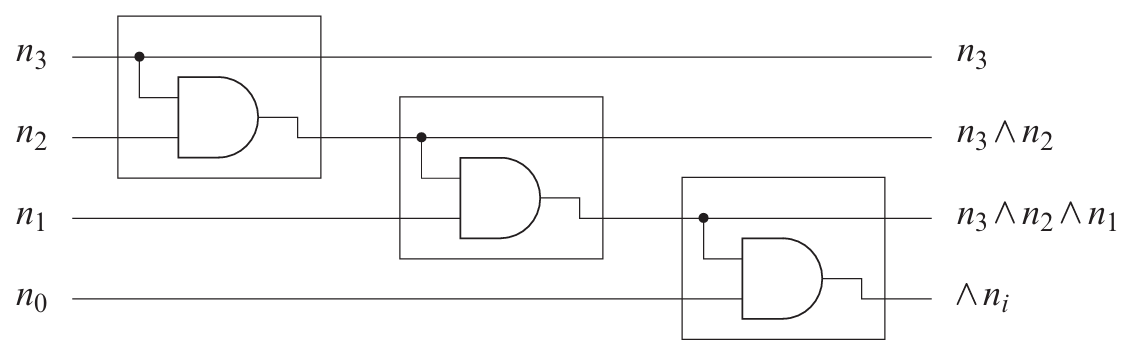
\includegraphics[width=0.5\linewidth]{Images/4bitconj.png}
    \caption{Irreversible Classical Circuit for four-bit conjunction}
    \label{fig:4bitconj}
\end{figure}
An arbitrary Boolean circuit can be transformed into a sequence of operations on a large enough register to hold input, output and intermediate bits. The space complexity of a circuit is the size of the register.

Computations performed by this machine are not reversible in general; by reusing bits in the register, the machine erases information that cannot be reconstructed later. A trivial, but highly space inefficient, solution to this problem is not to reuse bits during the entire computation. Figure \ref{fig:rev4bitconj} illustrates how the circuit can be made reversible by assigning the results of each operation to a new bit. The operation that reversibly computes the conjunction and leaves the result in a bit initially set to $0$ is, of course, the Toffoli gate. Since the NOT gate is reversible, and NOT together with AND form a complete set of Boolean operations, this construction can be generalized to turn any computation using Boolean logic operations into one using only reversible gates. This implementation, however, needs an additional bit for every AND performed, so if the original computation takes $t$ steps, then a reversible one constructed in this naive way requires up to $t$ additional bits of space.
\begin{figure}
    \centering
    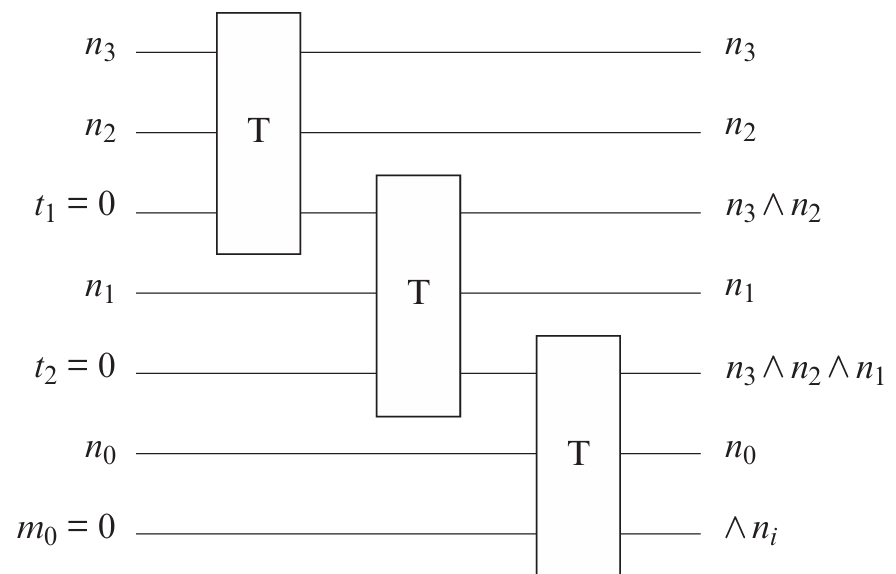
\includegraphics[width=0.5\linewidth]{Images/rev4bitconj.png}
    \caption{Reversible Classical circuit for four-bit conjunction}
    \label{fig:rev4bitconj}
\end{figure}
Furthermore, this additional space is no longer in the $0$ state and cannot be directly reused, for example, to compose two reversible circuits. Reusing temporary bits will be crucial to keeping the space requirements close to that of the original nonreversible classical computation. Resetting a bit to zero is not as trivial as it might seem. A transformation that reset a bit to $0$, regardless of whether it was $0$ or $1$ before, is not reversible (it loses information), so it cannot be used as part of reversible computation. Reversible computations cannot reclaim space through a simple reset operation. They can, however uncompute any bit set during the course of a reversible computation by reversing the part of the computation that computed the bit.

\begin{example}
    Consider the computation of figure \ref{fig:rev4bitconj}. Bits $t_1$ and $t_0$ are temporarily used to obtain the output in bit $m_0$. Figure \ref{fig:4bituncomp} shows how to uncompute these bits, resetting them to their original $0$ value by reversing all but the last step of the circuit in figure \ref{fig:rev4bitconj}, so that they may be reused as part of a continuing computation. Here the temporary bits are reclaimed at the cost of roughly doubling the number of steps.
\end{example}
\begin{figure}
    \centering
    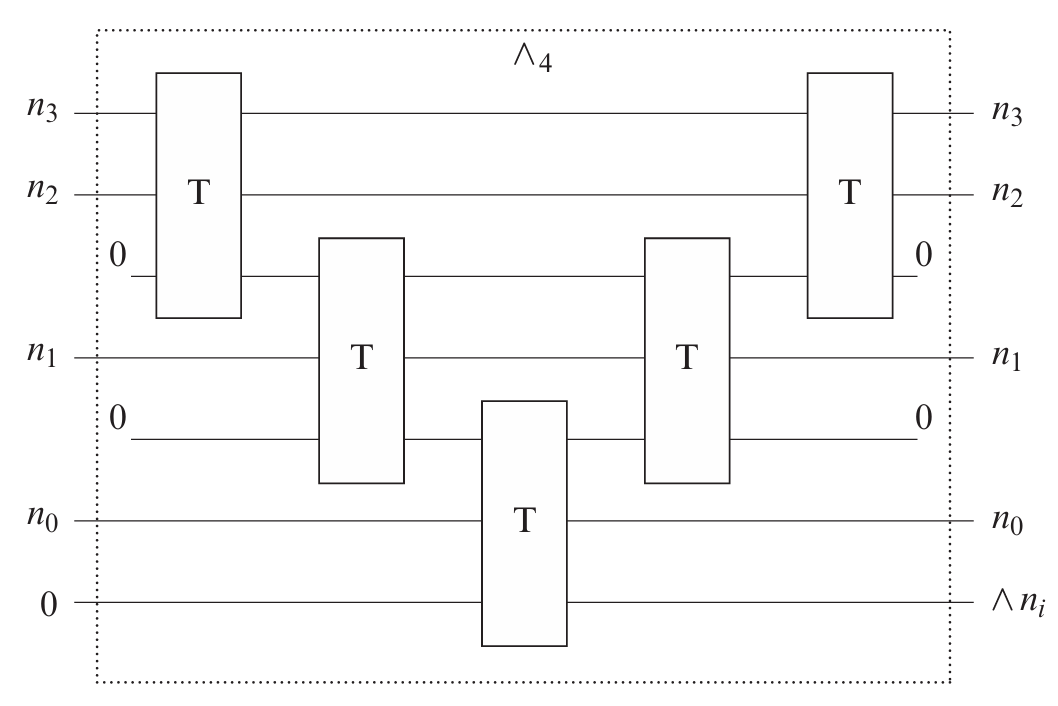
\includegraphics[width=0.5\linewidth]{Images/4bituncomp.png}
    \caption{Reversible Circuit that reclaims temporary bits}
    \label{fig:4bituncomp}
\end{figure}
We can reduce the number of qubits needed by uncomputing them and reusing them in the course of the algorithm. The method of uncomputing bits by eprforming all of these steps in reverse order, except those giving the output, works for any classical Boolean subcircuit. The naive construction requires up to $t$ additional bits in the register.

\begin{example}
    Suppose we want to construct the conjunction of eight bits. Simply reversing the steps, generalizing the approach shown in figure \ref{fig:4bitconj}, would require six additional temporary bits and one bit for the final output. We can save space by using the four-bit AND circuit of figure \ref{fig:4bituncomp} and then combining the results as shown in figure \ref{fig:8wayconj}. This construction uses two temporary bits in addition to the two temporary bits used in each of the four-bit ANDs. Since each of the four-bit ANDs uncomputes its temporary bits, these bits can be reused by the t four-bit ANDs. This circuit uses only a total of four additional temporary bits, though it does require more gates.
\end{example}
\begin{figure}
    \centering
    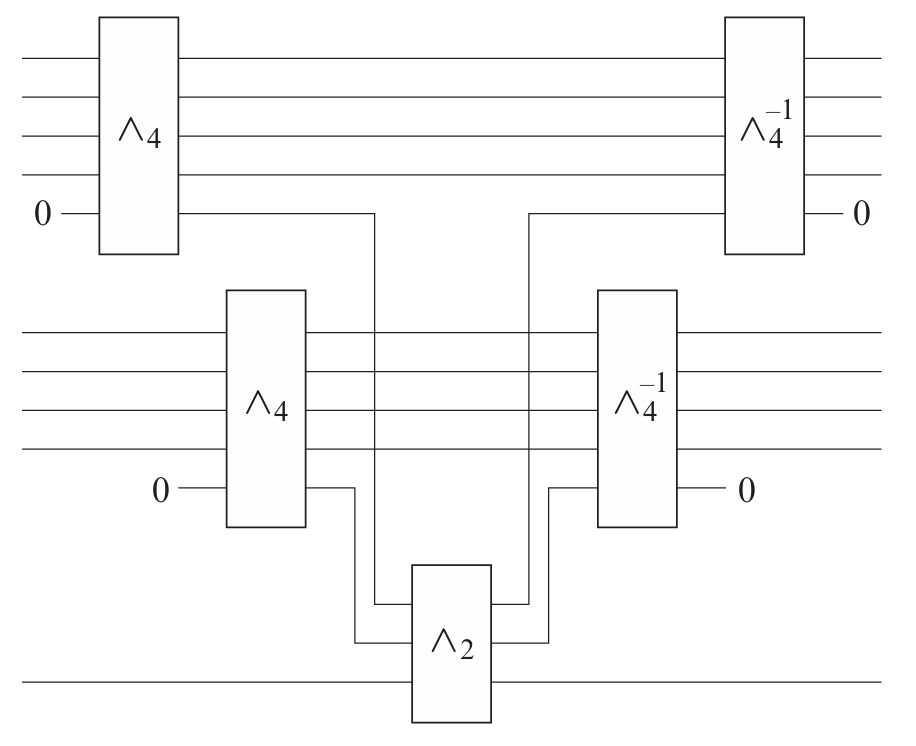
\includegraphics[width=0.5\linewidth]{Images/rev4bitANDS.png}
    \caption{Combining reversible 4-bit AND circuits of figure \ref{fig:4bitconj} to construct an eight-way conjunction}
    \label{fig:8wayconj}
\end{figure}
There is an art to deciding when to uncompute which bits to maintain efficiency and to retain subresults in the computation. The key ideas of this section, adding bits to obtain reversibility and uncomputing their values so that they may be reused, are the amin ingredients of the general construction. By choosing carefully when and what to uncompute, it is possible to make a positive tradeoff, sacrificing some additional gates to obtain a much more efficient use of space. Examples, such as an explicit implementation of an $m$-way AND.

\subsection{A General Construction}
This section shows how, by carefully choosing which bits to uncompute when, a reversible version of any classical computation can be achieved with only minor increases in the number of gates. We show that any classical circuit using $t$ gates and $s$ bits, has a reversible counterpart using only $O(t^{1+\epsilon})$ gates and $O(s\log t)$ bits. For $t>>s$, this construction uses significantly less space than the $(s+t)$ space of the naive approach described earlier at only a small increase in the number of gates.

In order to understand how to obtain these bounds, we must consider carefully how many bits are being used in what way. Let $C$ be a classical circuit, compose of AND and NOT gates, that uses not more that $t$ gates and $s$ bits. The circuit $C$ can be partitioned into $r=\lceil t/s\rceil$ subcircuits each containing $s$ or fewer consecutive gates $C=C_1C_2\ldots C_r$. Each subcircuit $C_i$ has $s$ input and $s$ output bits, some of which may be unchanged.

Using techniques from the previous section, each circuit $C_i$ can be replaced by a reversible circuit $R_i$ that uses at most $s$ additional bits as shown in figure \ref{fig:ctor}. The circuit $R_i$ returns its input as well as the $s$ output values in the subsequent computation. The input values will be used to compute and uncompute $R_i$ in order to save space.
\begin{figure}
    \centering
    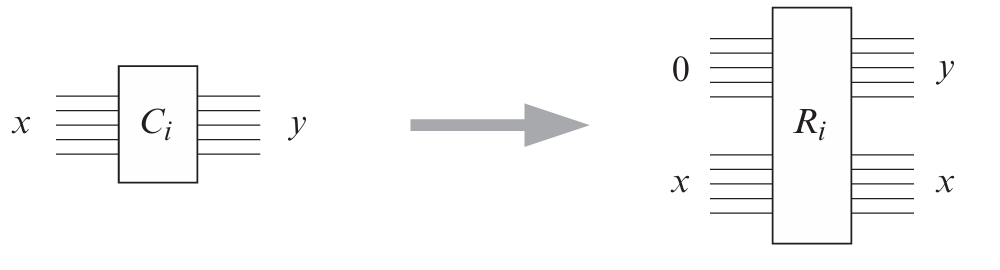
\includegraphics[width=0.5\linewidth]{Images/revector.png}
    \caption{Converting circuits $C_i$ to reversible ones $R_i$}
    \label{fig:ctor}
\end{figure}
More than $s$ gates may be required to construct $R_i$. In general, $R_i$ can be constructed using at most $3s$ gates. While other more efficient constructions are possible, the following three steps always work.
\begin{enumerate}
    \item \textbf{Step 1:} Compute all the output values in a reversible way. For every AND or NOT gate in the original circuit $C_i$, the circuit $R_i$ has a Toffoli or NOT gate. This step uses the same number of gates, $s$, as $C_i$, and uses no more than $s$ additional bits.
    \item \textbf{Step 2:} Copy all of the output values used in the subsequent parts of the computation, to the output register, a set of no more than $s$ additional bits. This is done using $s$ CNOT gates.
    \item \textbf{Step 3:} Perform the sequence of gates used to carry out step$1$, but this time in reverse order. In this way all bits, except those in the output register are set to their original values. Specifically, all temporary bits are returned to $0$, and we have recovered all of the input values.
\end{enumerate}
The circuits $R_1,\ldots,R_r$ when combined as in figure \ref{fig:rirevtoc}, perform the computation $C$ in reversible but space-inefficient way. The subcircuits $R_i$ can be combined in a special way that uses space more efficiently by uncomputing and reusing some of the bits. Uncomputing requires additional gates, so we must choose carefully when to uncompute in order to reduce the used of space without needing too many more gates. First, we show how to obtain a reversible version using $\mathcal{O}(t^{\log_2 3})$ gates and $\mathcal{O}(s\log t)$ bits , and then we improve upon this method to obtain $\mathcal{O}(t^{1+\epsilon})$ gates and $\mathcal{O}(s\log t)$ bit bounds.
\begin{figure}
    \centering
    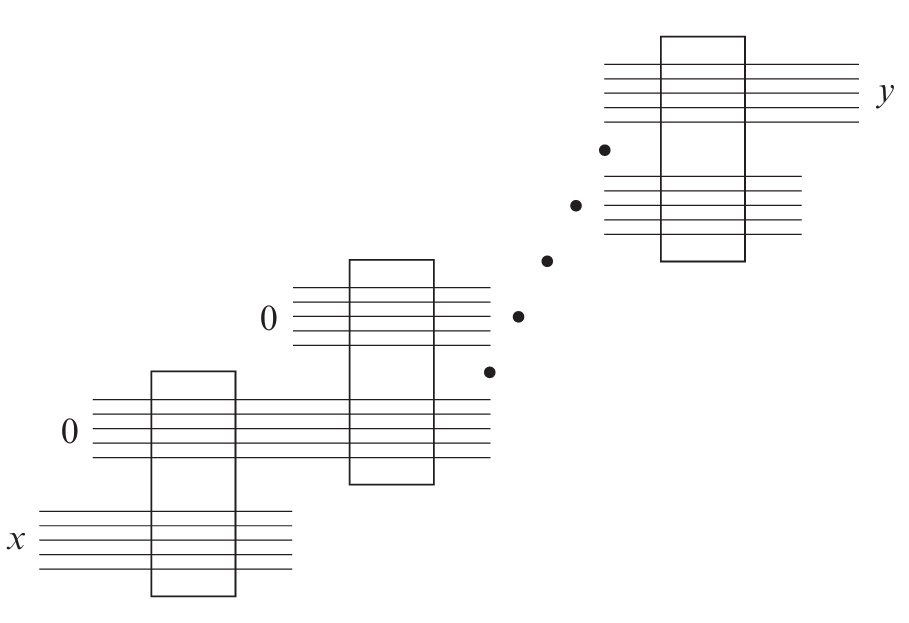
\includegraphics[width=0.5\linewidth]{Images/revcircr1torr.png}
    \caption{Composing the circuits $R_i$ to obtain a reversible, but inefficient, version of the circuit $C$}
    \label{fig:rirevtoc}
\end{figure}
To basic principle for combining the $r=\lceil t/s\rceil $ circuits $R_i$ is indicated in figure $\ref{fig:effimplertoc}$. The idea is to uncompute and recompute parts of the state selectively to reuse the space. We systematically modify the computation $R_1,R_2,\ldots R_r$ to reduce the total amount of space used and to reduce all the temporary bits to zero by the end of the computation.
\begin{figure}
    \centering
    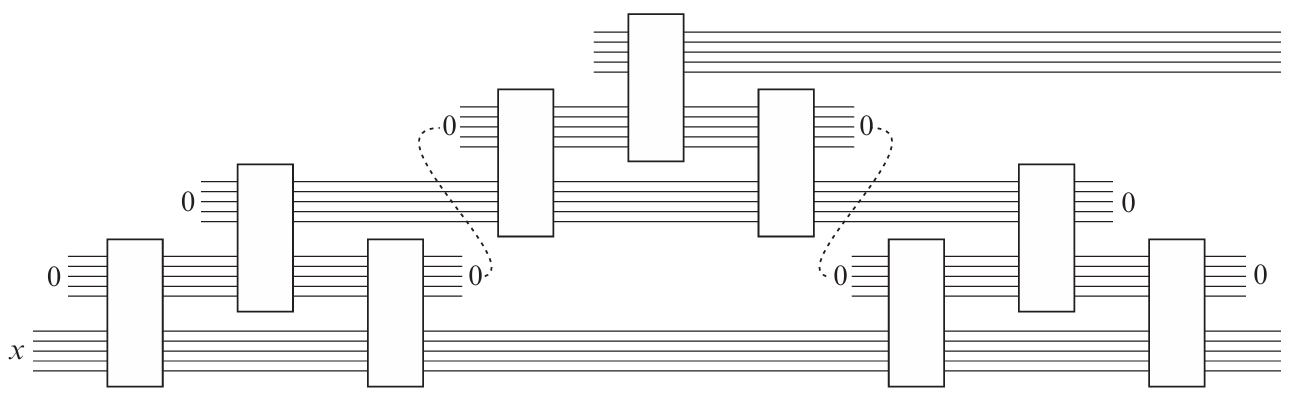
\includegraphics[width=0.75\linewidth]{Images/effimplertoc.png}
    \caption{Composition of reversible circuits $R_i$ in a way that reclaims storage}
    \label{fig:effimplertoc}
\end{figure}
To simplify the analysis, we take $r$ to be a power of two $r=2^k$. For $1\leq i\leq k$, let $r_i=2^i$. We perform the following recursive transformation $\mathcal{B}$ that breaks a sequence into two equal-sized parts, recursively transforms the parts, and then combines them in the way shown:
\begin{align*}
    \mathcal{B}(R_i,\ldots r_{i+1})&=\mathcal{B}(R_1,\ldots R_{r_i})\mathcal{B}(R_{1+r_i},\ldots ,R_{r_i+1})(\mathcal{B}(R_1,\ldots R_{r_i}))^{-1}\\
    \mathcal{B}(R)=R,
\end{align*}
where $(\mathcal{B}(R_1,\ldots,R_{t_i}))^{-1}$ acts non exactly the same bits as $\mathcal{B}(R_1,\ldots,R_{t_i})$ and so requires no additional space.

The transformed computation uncomputes all space except the output of the last step, so the additional space is bounded by $s$. Thus, $\mathcal{B}(R_1,\ldots, R_{r_i})$ requires at most $s$ more space than $B(R_1,\ldots,R_{r_i-1})$. We can write the space $S(i)$ required for each of the $k=\log_2 r$ steps $i$ in the recursion in terms of the space requirements of the previous step: $S\leq s +S(i-1)$ wth $S(1)\leq 2s$. The recursions ends after $k=\log_2 r$ steps, so the final computation $\mathcal{B}(R_1,\ldots,R_r)$ requires at mos $S(r)\leq (k+1)s=s(\log_2 r+1)$ space. From the definition of $\mathcal{B}$, it follows immediately that $T(i)$, the number of circuits $R_j$ executed by he computation $\mathcal{B}9R_1,\ldots, R_{r_i})$, is $T(i)=3T(i-1)$ with $T(1)=1$. By assumption $r=2^k$, so ther reversible version of $C$ we constructed uses
\[
T(2^k)=3T(2^{k-1})=3^k =3^{\log _2 r}=r^{\log _2 3}
\]
each of which requires fewer than $3s$ gates. Thus, any classical comptuation of $t$ steps and $s$ bits can be done reversibly in $O(t^{log_23})$ steps and $O(s\log_2 t)$ bits.

To obtain $O(t^{1+\epsilon})$ bound, instead of using a binary decomposition, consider the following m-ary decomposition. To simplify the analysis, suppose that $r$ is a power of $m$, $r=m^k$. For $1 \leq i\leq k$, let $r_i=m^{i}$. Abbreaviating $R_{1+(x-1)r_i,\ldots,R_{xr_i}}$ as $\vec{R_{x,i}}$, then
\begin{align*}
    \mathcal{B}(\vec{R}_{1,i+1})&=\mathcal{B}(\vec{R}_{1,i},\vec{R}_{2,i},\ldots,\vec{R}_{m,i})\\
    &=\mathcal{B}(\vec{R}_{1,i}),\mathcal{B}(\vec{R}_{2,i}),\ldots,\mathcal{B}(\vec{R}_{m-1,i}),\mathcal{B}(\vec{R}_{m,i}),\mathcal{B}(\vec{R}_{m-1,i})^{-1},\ldots,\mathcal{B}(\vec{R}_{2,i})^{-1},\mathcal{B}(\vec{R}_{1,i})^{-1}\\
    \mathcal{B}(R)&=R
\end{align*}
In each step of the recursion, each block is split into $m$ pieces an replaced with $2m-1$ blocks. We may assume without loss of generality that $r=m^k$ for some $k$, in which case we stop recursing after $k$ steps. At this point $r=m^k$ subcircuits $C_1$ have been replaced by $(2m-1)^k$ reversible circuits $R_i$, so thet taotal number of circuits $R_i$ for the final computation is $(2m-1)^k$, which we rewrite in terms of $r$:
\[
(2m-1)^{\log_m r}=r^{\log_m (2m-1)}\approx r^{\log_m2m}=r^{1+\frac{1}{\log_2 m}}
\]
The number of primitive gates in $R_i$ is bounded by $3s$ and $r=\lceil t/s\rceil$. The total number of gates for a reversible circuit of $t$ gates is 
\[
T(t)\approx 3s\left(\frac{t}{s}\right)<3t^{1+\frac{1}{\log_2m}}
\]
Thus, for any $\epsilon>0$, it is possible toc hoose $m$ sufficiently large that the number of gates required for the reversible computation is $\mathcal{O}(t^{1+\epsilon})$. The space bound remains the same as before $\mathcal{O}(s\log_2 t)$.

Reversible versions of classical Boolean constructed int his manner an be turned directly into quantum circuits consisting entirely of Toffoli and X gates. While our argument was given in terms of Boolean circuits, Bennet used the sam argument to show that any classical Turing machine can be turned into a reversible one. Based on these arrangements, from any classical circuit for $f$, an implementation of $U_f$ can be constructed of comparable number of gates and bits.

The care needed in uncomputing and reusing bits generalizes where the need for uncomputing values is even greater; uncomputing ensures that temporary qubits are no longer entagled with output qubits. This need to unentangle temporary values at the end of a computation is one of the differences between classical and quantum implementations. Quantum transformations, being reversible, cannot simply reset qubits. Naively, one might think that temporary qubits could be reset by measuring the qubit and then, depending on the measurement outcome, performing a transformation to set them to $\ket{0}$. But if the temporary qubits were entangled with qubits containing the desired result, or results used later in the computation, measuring the temporary qubits may alter those results. Uncomputing temporary qubits disentangles them from the rest of the system without affecting the state of the rest of the system. In the next section we give a number of examples of uncomputing temporary qubits.
The next section is to describe explicit implementations of certain arithmetic functions. These implementation are often more efficient than the general construction just given, but they all have analogous classical implementations of comparable efficiency.

The programs in this section implement quantum circuits for modular arithmetic and supporting operations, The operations shown are more general (though less efficient) than the modular arithmetic implementations used as part of Shor's algorithm; here the modulus, $M$, is placed in a quantum register so these algorithms can act on superpositions of different moduli as well as on superpositions of the input.

\subsection{Efficient implementation of AND}
We give a linear implementation of an m-way AND computed into an output qubit using just one additional temporary qubit.

\subsection{The Implementations}
We now describe quantum implementations for some specific arithmetic functions. When we talk about the efficiency of these implementations, we simply count the number of simple gates in the quantum circuits they describe. This quantity is called the circuit complexity. Note that in the classical case a quantum circuit for adding $24$-bit numbers differs from a circuit for adding $12$-bit numbers, though they may be related. 

\subsubsection{Integer Addition}
\textbf{Input: $x,y\in \mathbb{Z}$}\\
\textbf{Output: $x+y$}\\

One can formalize the notion for an efficient algorithm for a given problem in various ways by describing precise models of computation. For the purposes of this discussion let us just think in terms of Boolean circuits and identify an algorithm with a collection of acyclic circuits (one for each possible input length) that produce the correct outputs for all possible input strings. The circuits should be composed of $AND,OR,$ and $NOT$ gates, along with FANOUT operations (which we would often not consider as gates at all), and in order to be considered efficient, the total number of gates in each circuit should be polynomial in the number of input bits.

The number of bits needed to write down the number $x$ in binary notation is
\[
lg(x)=\begin{cases} 1 & \text{if } x=0 \\ \lfloor \log_2 |x|\rfloor+2 & \text{if } x \neq 0 \end{cases}
\]
assuming we keep a sign bit for each non-zero integer, and so the number of input bits of the above problem is $\log_(x)+\log_(y)$. Now, if you consider the usual method for adding number that you probably learned in elementary school or before, but using base 2 instead of base 10, you could turn that method into a construction of Boolean circuits of size $O(\log_(x)+\log_(y))$ for solving this problem. This is in fact linear in the input size, and so this algorithm will be considered to be very efficient.

By the way, I should mention that it is typical to place additional constraints on collections of Boolean circuits in order for the circuits to be identified with efficient algorithms. In particular, the circuits should satisfy certain uniformity constraints, which means that not only do they have polynomial size, but moreover there should not exist an efficient construction of the circuits themselves. This issue can be ignored in this class, however.

Summing up, we would simply say that the Boolean circuit complexity, or ``bit complexity" of computing $x+y$ for integers $x$ and $y$ is $\mathcal{O}(\log_2 x + \log_ y)$. Or even more simply, the bit complexity of adding two n bit integers is $\mathcal{O}(n)$.
Here are some other arithmetic and number theoretic problems:

\subsubsection{Integer Multiplication}
\textbf{Input: $x,y \in \mathbb{Z}$}\\
\textbf{Output: $xy$}

The ``elementary school" multiplication algorithm established that the bit complexity of multiplying $x$ and $y$ is $O((lg x)(lg y))$, or more simply that the bit complexity of multiplying two n bit numbers if $O(n^2)$. In fact, there are asymptotically better methods, such as the Schonhage-Strassen Algorithm that has bit complexity $O(n\log n \log \log n)$. (Large constant factors in the running time make this particular method less efficient than other methods until $n$ becomes quite large - several thousand bits perhaps.)

\subsubsection{Integer Division}
\textbf{Input: Integers $x$ and $y\neq 0$}\\
\textbf{Output: Integers $a$ an $b$, with $0\leq |y|$ such that $x=ay+b$}

 The cost is roughly the same as integer multiplication - the ``elementary school" division method gives an algorithm with bit complexity $O((\log_2 x)(\log_2 y))$. (in fact it is actually somewhat better: $O((\log_2 a)(\log_2 b))$.)

\subsubsection{Greatest Common Divisor}
\textbf{Input: Non-negative integers $x$ and $y$}\\
\textbf{Output: $gcd(x,y)$}

Euclid's algorithm, which is over 2000 years old, computes $gcd(x,y)$ in $O((\log_2 x) (\log_2 y))$ bit operations.

\subsubsection{Modular Integer Addition}
\textbf{Input: A positive integer $N$ and integers $x,y \in \mathbb{Z}_N = \{0,\ldots,N-1\}$}\\
\textbf{Output: $x+y \text{mod $N$}$}

The bit complexity of this problem is $O(\log_2 N)$.

\subsubsection{Modular integer Multiplication}
\textbf{Input: A positive integer $N$ and integers $x,y \in \mathbb{Z}_N$}\\
\textbf{Output: $xy \text{(mod N)}$}

Here the bit complexity is $O((\log_2 N)^2)$ by the elementary school algorithm, again asymptotically faster methods exist.

\subsubsection{Modular Inverse}
\textbf{Input: A positive integer $N$ and an integer $x \in \mathbb{Z}_N^*=\{a\in\mathbb{Z}_N: gcd(a,N)=1\}$}.\\
\textbf{Output: $y \in \mathbb{Z}_N$ such that $xy=1 \text{ (mod N)}$}

The bit complexity is $O((\log_2 N)^2)$.

\subsubsection{Modular Exponentiation}
\textbf{Input: A positive integer $N$, an integer $x \in \{0,\ldots,N-1\}$, and any integer $k$.}\\
\textbf{Output: $x^k$ (mod N)}

Using the method of repeated squaring, the bit complexity is $O((\log_2 k)(\log_2N)^2)$.

\subsubsection{Primality testing}
\textbf{Input: A positive integer $N$}\\
\textbf{Output: ``prime" if $N$ is a prime number, ``not prime" otherwise.}

Randomized algorithms having bit complexity $O((\log_2 N)^3)$ that allow a probability $1/4$, say, of making an error have been known for many years. In a breakthrough a few years ago, Agarwal, Kayal and Saxena gave a deterministic prime testing algorithm that gives a $O((\log_2 N)^6)$ deterministic algorithm for testing primality.

\subsubsection{Integer Factoring}
\textbf{Input: A positive integer $N$}\\\
\textbf{Output: A prime factorization $N=P_1^{a_1}\ldots p_k^{a_k}$ of $N$}

No classical algorithm is known to give a polynomial bit complexity of factoring - the best known algorithm asymptotically gives a bit complexity of

\[
2^{O((\log N)^{1/3}(\log \log N)^{2/3})}
\]
We will see that when we turn to quantum algorithms, Shor's algorithm will solve the Integer Factoring problem using $O((\log_2N)^3)$ operations, giving a remarkable speed-up over known classical algorithms for this task.


\section{Complexity of Quantum Algorithms}
\begin{definition}
    \textbf{Efficiency of Quantum Algorithm: } Let $n$ be the number of input bits. A Quantum Algorithm is efficient if the number of gates in the quantum circuit is $\mathcal{O}(poly(n))$.
\end{definition} 

\begin{definition}
    \textbf{Probabilistic nature of quantum algorithms:} Because of Probabilistic nature of measurements it is required for probability of correct answer to be higher. Generally, $p>2/3$ is considered to be a good probability of success or at least $p>1/2 + 1/poly(n)$. Consider a case when Probability of getting a correct answer is $p=1/2+\epsilon$ where $\epsilon>0$ is a constant. Then the best method of deciding the correct answer is based on the frequency of the outcomes, the higher frequency outcome is the correct answer. But how many repetitions should be performed? Then the number of repetitions of the algorithm can be found using Chernoff bound as (say for binary outcome $X_i=0$ or $X_i=1$):
\[P(\sum X_i \leq n/2) \leq e^{-2n\epsilon^2}\] 
where n is the number of times. Thus the error gets exponentially small.
\end{definition}

\begin{definition}
    \textbf{(Computational Cost/Query Complexity):}
    In Quantum Algorithms, Computational cost is equal to the Query Complexity. The query complexity is the number of times we call the query oracle ($U_f$).
\end{definition}
The goal is to perform a given task using as few queries as possible to oracle ($U_f$). A Quantum Oracle (black box) is a Unitary operator that implements the function $f$.

\begin{example}
    (Query access to boolean function) $f:\{0,1\}^n \rightarrow \{0,1\}$ be a boolean function and oracle be defined as:
    \[ U_f\ket{x}=(-1)^{f(x)}\ket{x} \]
    where $x \in \{0,1\}^n$. This is used in Grover's Algorithm. This is called phase kickback as $f(x)$ is returned as a phase factor.
    Thus, $U_f$ can be applied to superposition of the states in computational basis.
    Having query access to $f(x)$ does not mean we know $f(x)$.
\end{example}
\begin{example}
    (Partially specified oracles) Sometimes it is possible we might not be interested in entire $U_f$ but only $U_f$ applied to certain vectors
    say for example, as shown
    \[ U_f\ket{0}\ket{x}=\ket{0}A\ket{x}+\ket{1}B\ket{x}\]
    \[U_f=\begin{bmatrix} A & * \\ B & * \end{bmatrix}\]
    where $A,B$ are arbitrary $ N \times N$ unitary matrices. This is called as partially specified oracle.
\end{example}

Query complexity hides the implementation details of $U_f$. For some cases, we can prove lower bounds on number of queries to solve a certain problems (example: Grover's Algorithm) but it's a difficult problem. 
\begin{definition}
    \textbf{(Gate Complexity):} The number of \textit{elementary gates} needed to implement the oracle $U_f$.
\end{definition}
Some queries can be (provably) difficult to implement, and there can be a large gap between the query complexity and gate complexity. \textbf{Quantum Algorithm should not dominate the total gate complexity.}
\begin{definition}
    \textbf{(Circuit Depth):}
    Circuit depth is the maximum number of gates on any path from input to output. It is equivalent of ``Wall clock time" in classical computation.
\end{definition} 

\begin{definition}
    \textbf{(Coherence Time):} Quantum states can be preserved only for a short amount of time called coherence time.
\end{definition}
Thus circuit depth can be used to check whether the coherence time is exceeded by a Quantum Computer.

Quantum Algorithms should be depth efficient. Thus, try to reduce the circuit time even if we need to run it multiple times.

A Quantum Algorithm consist of set of qubits (system registers - storing quantum states of interest and ancilla registers - 
auxiliary registers needed to implement the unitary operations acting on system registers) starting from an initial state, apply a series of one/two qubit states, and perform measurements, perform uncomputation whenever possible.
\begin{definition}
    \textbf{(Working Register):} Within ancilla register if a register can be freed by uncomputation then it is called a working register. Working register can be reused for other purposes.
\end{definition}
Note that we do not factor the cost of working registers into asymptotic cost analysis in the literature.

\section{Oracles}\label{sec:Oracles}
Before jumping into Quantum Algorithms we must understand the Oracles and their working.
Consider a classical circuit representing a classical function $f$. 
Consider the classical function $f:\{0,1\}^n \rightarrow \{0,1\}^m$ which takes $n$ bits as input and gives $m$ bits as output.
\textbf{We can represent this classical function using a classical circuit}. (For the proof of this please refer to Appendix \ref{proof:classicalcomputations})
Thus, any classical boolean function $f:\{0,1\}^n \rightarrow \{0,1\}^m$ can be represented using a classical circuit as shown in the figure \ref{classicalcircuit}.
\begin{figure}[ht]
    \centering
    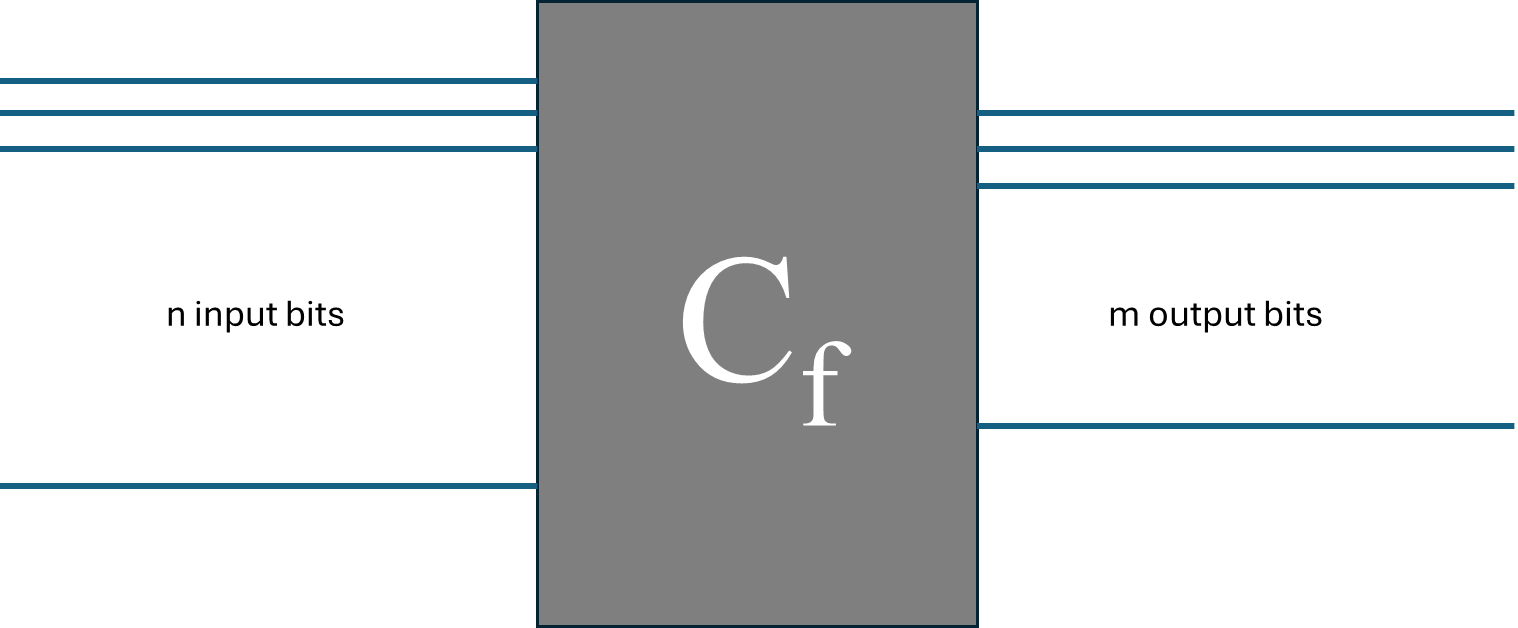
\includegraphics[width=0.8\textwidth]{Images/classicalcircuit.png}
    \caption{Classical Circuit}
    \label{classicalcircuit}
\end{figure}
But we are interested in Quantum Circuits. Thus, we are required to convert this classical circuit into a Quantum Circuit.
Recall, that a Quantum Circuit is a sequence of Quantum Gates. Since all the operations using quantum gates done on qubits  are untiary opertaions (thus, reversible),
and thus the Quantum circuit can be written as a product of Unitary quantum gates which is a Unitary matrix (product of unitary matrices is a unitary matrix). Thus, the Quantum Circuit is itself a Unitary Gate and hence reversible. Thus, the Quantum circuits are reversible.
Note that here the meaning of reversibility is that given the output of the circuit we can find the input of the circuit. This is because the Quantum Gates are Unitary and thus reversible.
Thus, a Gate is said to be reversible if given the output of the gate we can find the input of the gate. 

But, a classical circuit need not be necessarily reversible. Thus, we are required to convert the classical circuit into a reversible circuit in order to implement it on a Quantum Computer as a Quantum Circuit (Unitary Gates i.e. hence always reversible).
Thus, we are required to transform the classical circuit in order to make it reversible in order to implement it as a Unitary matrix made up of Quantum Gates (reversible since $U_f^{\dagger}=U_f^{-1}$).

This, can be done by transforming gates in a classical universal gate set to corresponding reversible quantum gates. Thus, then can we implement any classical circuit on a quantum computer. 
Note that a universal gate set is the set of gates which can be used to implement any classical circuit. There can be multiple gate set which form the universal gate sets. For example, the $\{NAND\}$ gate is a universal gate set,
$\{AND, NOT\}$ is another universal gate set. Thus, we can create any classical circuit using only the gates in the universal gate set. Now, if we are able to show that 
the gates in the universal gate set can be transformed into reversible quantum gates, then we can implement any classical circuit on a quantum computer using the corresponding reversible quantum gates. We can convert any classical circuit in terms of the universal gate sets and then 
replace the gates in the universal gate set with their corresponding reversible quantum gates to get the quantum circuit.

For the consideration let us take the Classical universal gate set $\{AND,NOT\}$. Here, NOT gate (refer Appendix \ref{cgate:NOT}) is already reversible 
becuase if we know the output of the NOT gate we can find the input. For example, if the output of the NOT gate is 1 then we know that the input was 0 and if the output of the NOT gate is 0 then we know that the input was 1. This is because NOT is a single input single output gate (number of inputs=number of outputs)
which negates the input. Thus, for the two inputs $0$ and $1$ we get the outputs $1$ and $0$ respectively. Thus, for finding the input from the given output we can simply negate that output to get the input (negation twice cancels out). Hence, the NOT gate is already a reversible gate. 
It's equivalent Quantum Gate is the Pauli-X gate which is also reversible. Thus, we can replace the NOT gate in the classical circuit with the Pauli-X gate in the Quantum Circuit.
Recall that the Pauli-X Gate is $\begin{bmatrix} 0 & 1 \\ 1 & 0 \end{bmatrix}$ and its action on $\ket{0}$ and $\ket{1}$ are $X\ket{0}=\ket{1}$ and $X\ket{1}=\ket{0}$
respectively. Thus, the Pauli-X gate is reversible and the quantum equivalent of the Classical NOT Gate.

Now, we are left with the AND gate. The AND gate is a two input single output gate i.e. It takes two inputs and gives one output. The output is 1 if and only if both the inputs are 1, else the output is 0 (refer Appendix \ref{cgate:AND}).
Thus, for the case when the output is 0 the input could be either $00$ or $01$ or $10$ but not $11$. For the output of 1 we definitely know that the input was $11$. 
But, for the output of $00$ we cannot determine the input. Thus, the AND gate is not reversible. Thus, we are required to convert the AND gate into a reversible gate in order to implement it on a Quantum Computer.
Thus, in order to create a reversible AND gate consider the control-Swap Gate (refer section \ref{qgate:cswap}). It takes three different inputs say
$\ket{x}$, $\ket{y}$ and $\ket{z}$. Say x acts as the control bit and y and z are the target bits. 
This, is as shown in the figure \ref{fig:cswap}
\begin{figure}[ht]
    \centering
    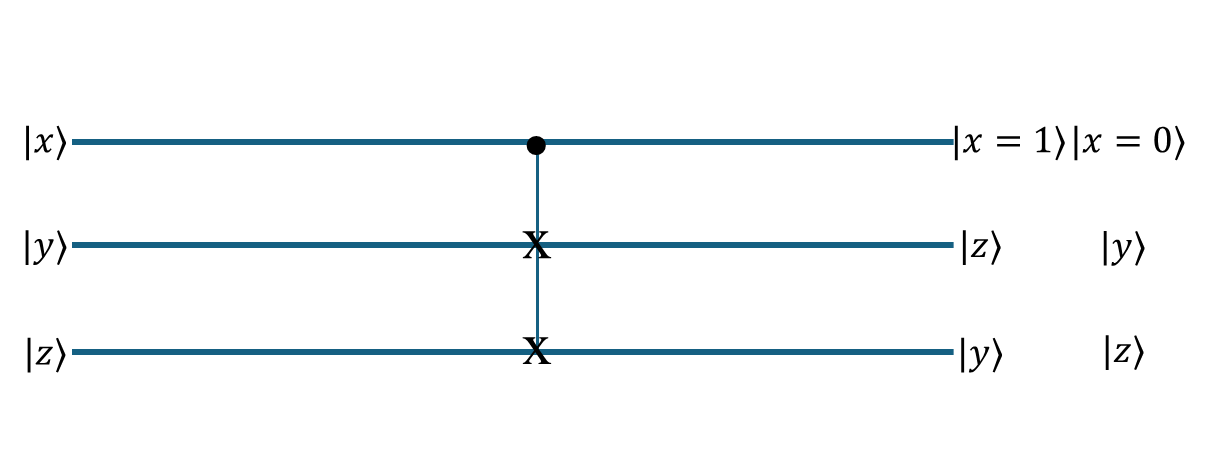
\includegraphics[width=0.8\textwidth]{Images/reversiblecswap.png}
    \caption{Control Swap Gate}
    \label{fig:cswap}
\end{figure}
Thus, if 
$x=1$ then the state of the system is swapped i.e. $\ket{y}$ and $\ket{z}$ are swapped, thus the output is $\ket{x},\ket{z},\ket{y}$. If $x=0$ then the state of the system remains the same $\ket{x},\ket{y},\ket{z}$.

Now in order to create reversible AND gate using the control-Swap gate we can do the following. Set the $\ket{z}=\ket{0}$.
Then, the output of the control-Swap gate will be $\ket{x},\ket{0},\ket{y}$ if $x=1$ and $\ket{x},\ket{y},\ket{0}$ if $x=0$.
This, output can also be written in a more compact form as $\ket{x},(\ket{0},\ket{y}),\ket{x \land y}$ where $\land$ is the AND operation. The second qubit can be either $\ket{0}$ or $\ket{y}$ depending on the value of $x$.
If $x=1$ then the second qubit will be $\ket{0}$ and if $x=0$ then the second qubit will be $\ket{y}$. This, output of the second qubit is referred to as junk which is a function of x i.e. $junk(x)$. This is as shown in the figure \ref{fig:reversibleand}.
\begin{figure}[ht]
    \centering
    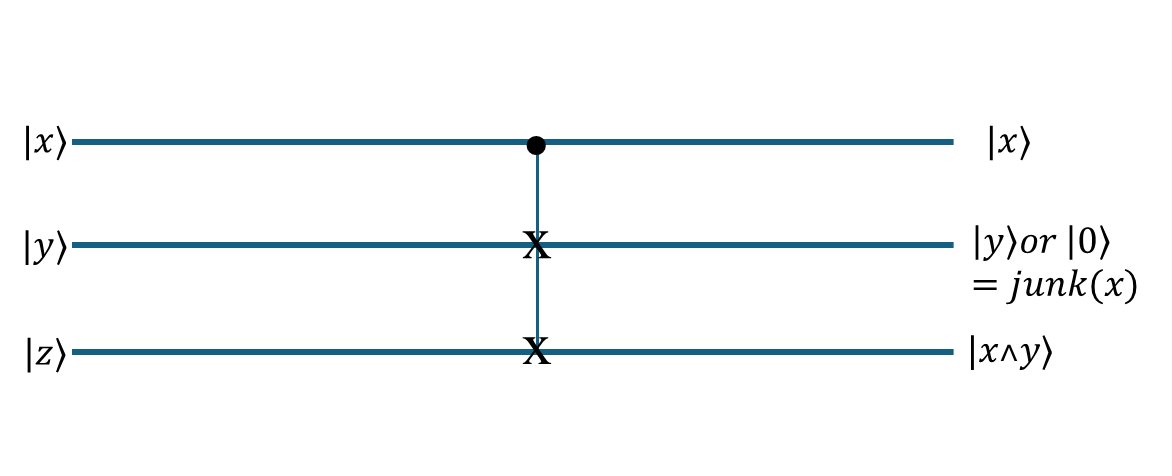
\includegraphics[width=0.8\textwidth]{Images/reversibleand.png}
    \caption{Reversible AND Gate}
    \label{fig:reversibleand}
\end{figure}
The truth table for the above circuit is as shown in the table \ref{tab:reversibleand}.
\begin{table}[ht]
    \centering
    \begin{tabular}{|c|c|c|c|c|}
        \hline
        $x$ & $y$ & $0$ & $junk(x)$ & $x \land y$ \\
        \hline
        0 & 0 & 0 & 0 & 0 \\
        0 & 1 & 0 & 1 & 0 \\
        1 & 0 & 0 & 0 & 0 \\
        1 & 1 & 0 & 0 & 1 \\
        \hline
    \end{tabular}
    \caption{Reversible AND Gate}
    \label{tab:reversibleand}
\end{table}
Hence, we can clearly see that the output of the circuit is the same as the output of the AND gate. Thus, the above circuit is the reversible AND gate. 
Thus, using CSWAP gate as shown above we can convert the AND gate into a reversible gate. 

Thus, we can convert any classical circuit into a reversible circuit by replacing the gates in the universal gate set with their corresponding reversible quantum gates.
We replace NOT gate with the Pauli-X gate and the AND gate with the modified CSWAP Gate. 
Hence, any classical function can be implemented on a classical circuit (in terms of universal gate set $\{AND,NOT\}$) which then can be converted to a reversible circuit by replacing the gates in the universal gate set with their corresponding reversible quantum gates
($AND$ gate with Modified CSWAP and NOT gate with Pauli-X gate). Thus, for a general classical function with corresponding implementation in classical circuit as $C_f$ we would have a corresponding
quantum circuit $U_f$ which is the reversible version of the classical circuit $C_f$ thus, implementing the classical function $f$ on a quantum circuit by making it reversible. Here, we have converted the classical function $f$ to a reversible function $\tilde{f}$ which has number of inputs equal to the number of outputs, 
produces the same output as the classical function $f$ along with the input and some junk values as shown in the figure \ref{fig:classicaltoquantum}. \textbf{We can implement any classical function on a quantum circuit.}
\begin{figure}
    \centering
    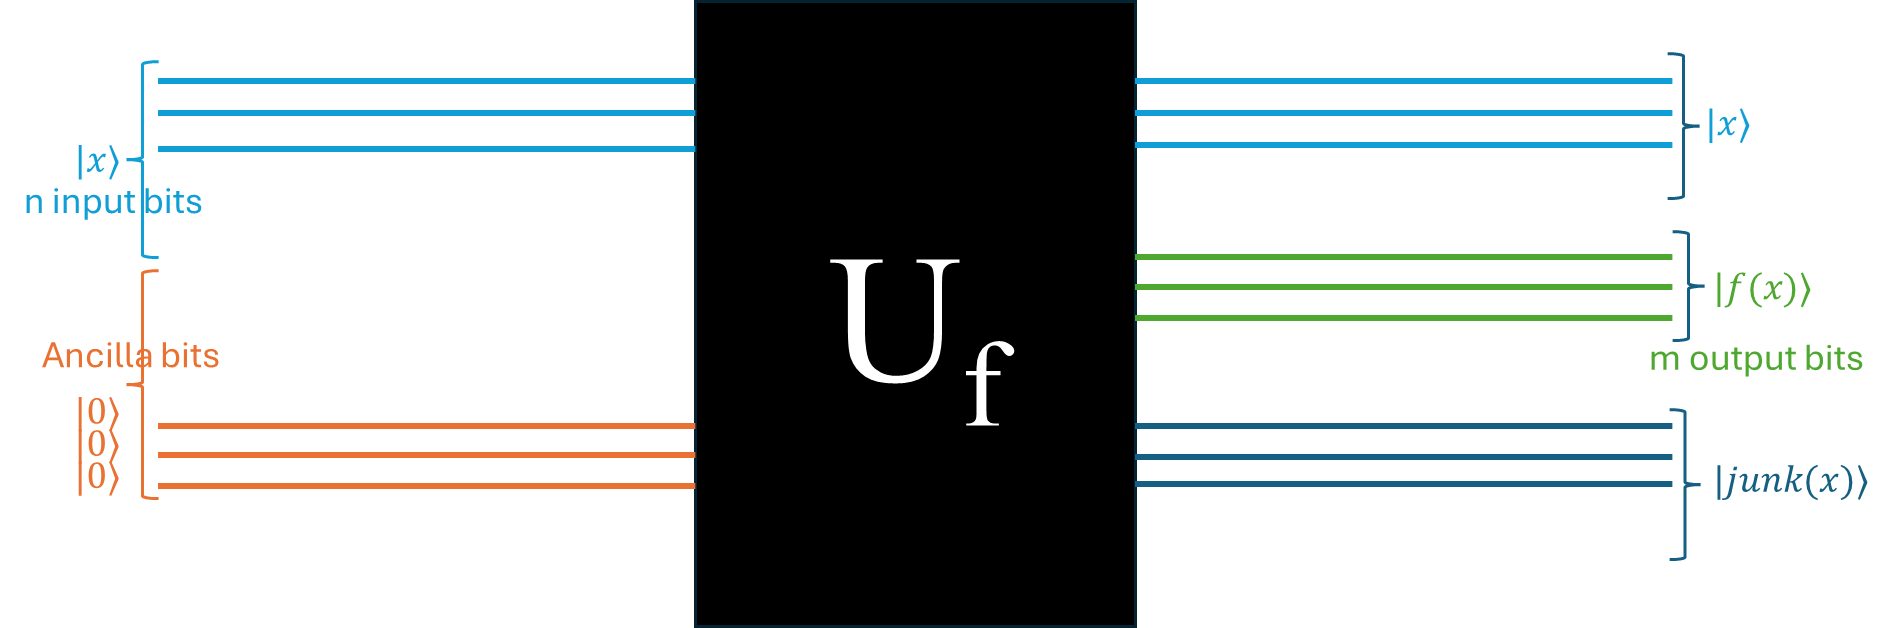
\includegraphics[width=0.8\textwidth]{Images/classicaltoquantum.png}
    \caption{Quantum Circuit}
    \label{fig:classicaltoquantum}
\end{figure}
The above figure shows the conversion of a classical circuit to a quantum circuit. 

Thus, a classical circuit when converted to a quantum circuit is as shown in the figure \ref{fig:classicaltoquantum}, it takes input $\ket{x}$ and along with it 
some ancilla bits (aka junk bits) and produces the output $\ket{x}$, $\ket{y \oplus f(x)}$ along with some junk bits $junk(x)$. We need to remove the junk since it consumes extra amount of qubits which is a waste of quantum resources and 
also the junk bits might get entangled with the output and any interference with environment may lead to decoherence or incorrect output and errors. Thus, we need to remove the junk bits.
This is done using the following circuit \ref{fig:quantumoracle}
\begin{figure}[ht]
    \centering
    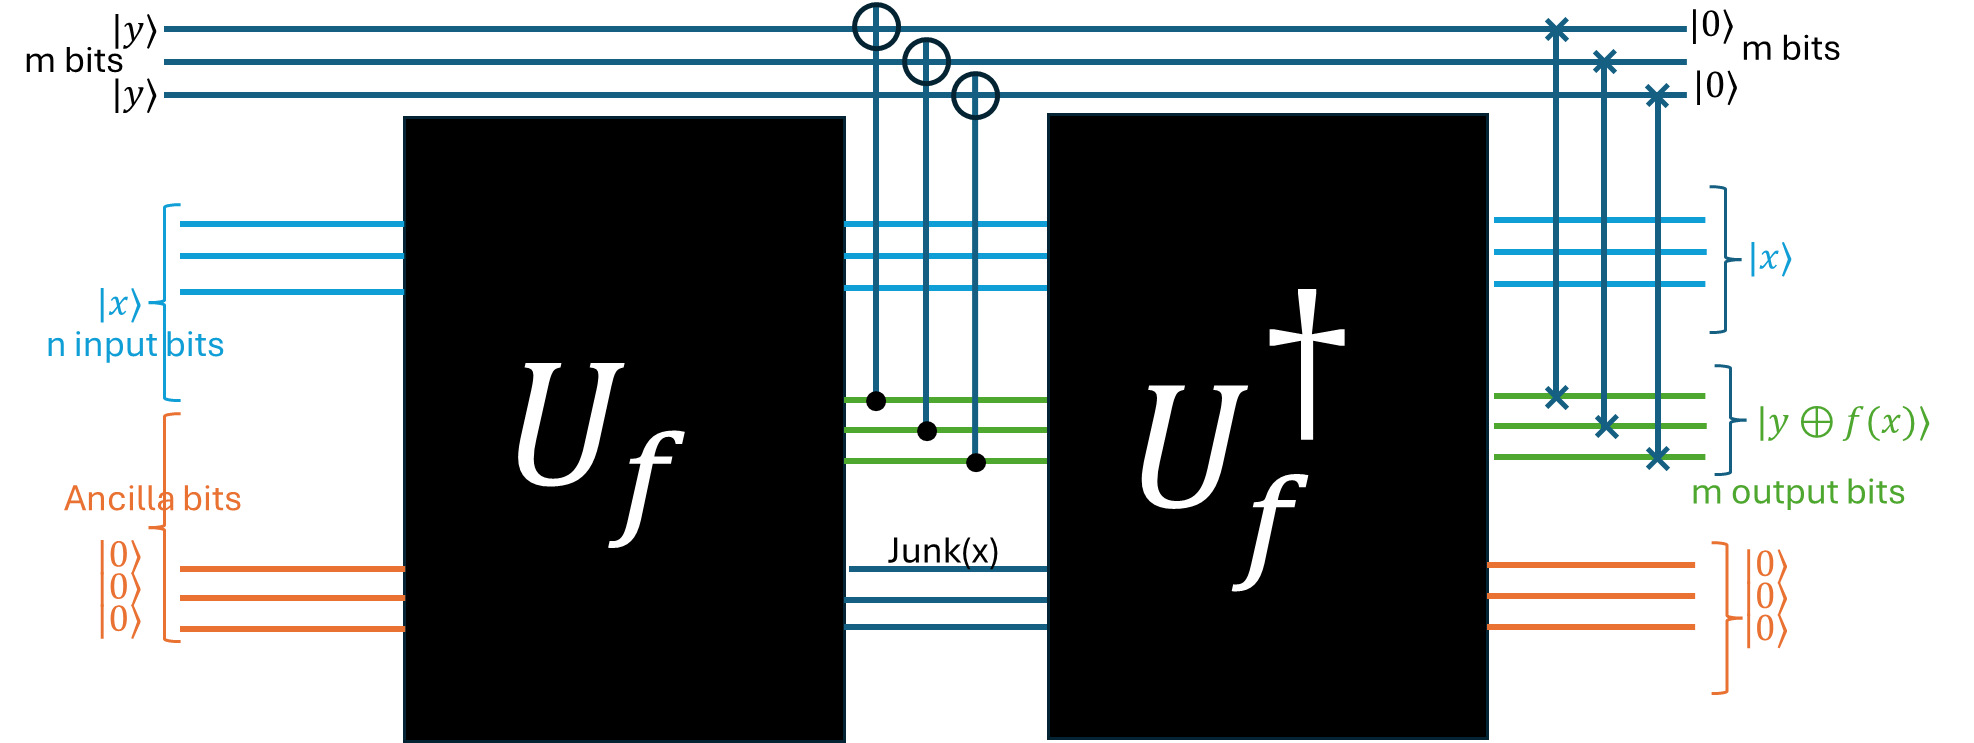
\includegraphics[width=0.8\textwidth]{Images/quantumoracle.png}
    \caption{Quantum Oracle}
    \label{fig:quantumoracle}
\end{figure}
Using this circuit it can be seen that the output of the entire circuit is $\ket{x},\ket{y\oplus f(x)}$ and the junk bits are are now $\ket{0}$ so that they can be used for other purposes in the circuit ahead. 
The output from the first Quantum Circuit $U_f$ is $\ket{x},\ket{y\oplus f(x)},junk(x)$. To remove the junk bits, it was done by first copying the output $\ket{f(x)}$ to the other (working bits) bits and then the output from the $U_f$ circuit was passed through its inverse $U_f^{-1}=U^{\dagger}_f$. Thus, upon passing through its inverse the output will be $\ket{x},\ket{0},\ket{0}$ since $U_f^{\dagger}$ is a reverse circuit and hence will make the outputs back to the inputs. 
Then the bits are swapped between as shown in the figure to get the desired output of 
$\ket{x},\ket{y\oplus f(x)},\ket{0},\ket{0}$ with no junk. Thus, the output of the circuit is the input $\ket{x}$ and the output $\ket{y\oplus f(x)}$. This entire thing is called an Oracle. 
Thus, we can imagine a Quantum Circuit which is an implementation of a classical function $f$ as a black box which takes input $\ket{x}, \ket{y},\ket{0}$ and produces the output $\ket{x},\ket{y\oplus f(x)},\ket{0}$. 
For the sake of simplicity we generally ignore the $\ket{0}$ in inputs and outputs. 

Thus, whenever given a classical function $f$, we can make it as a reversible quantum function and thus, implement
it as a quantum circuit using reversible quantum gates. This can be visualized as shown in the figure \ref{oracle}.
\begin{figure}[ht]   
    \centering
    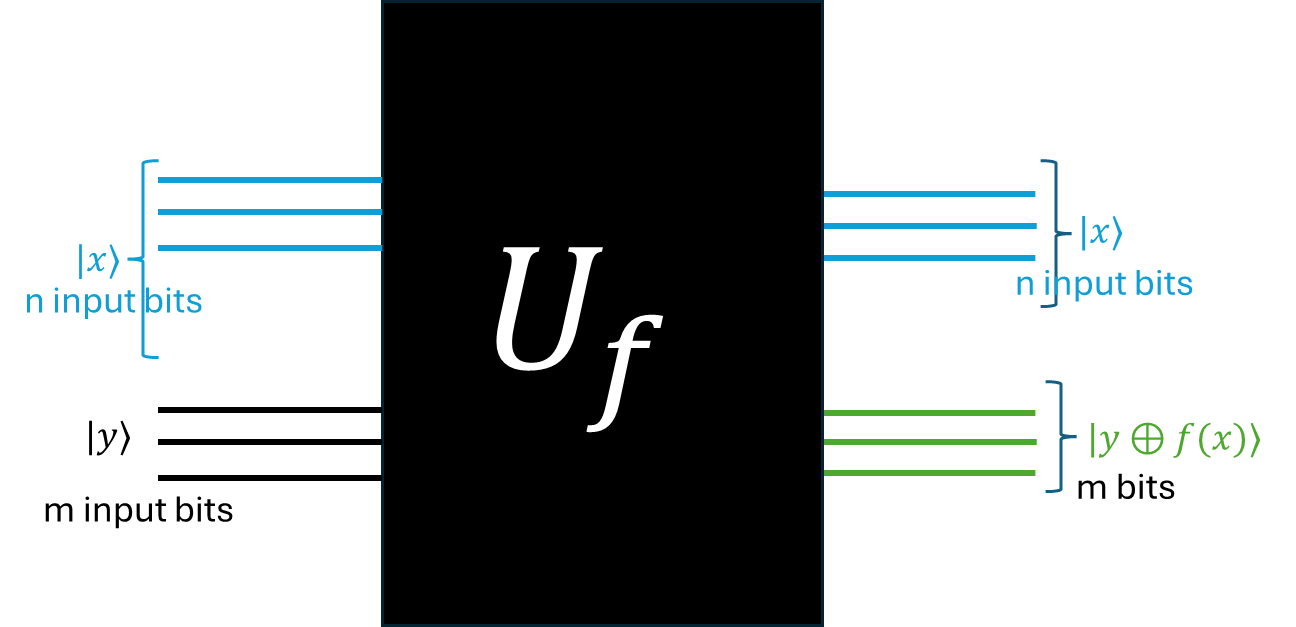
\includegraphics[width=0.8\textwidth]{Images/oracle.png}
    \caption{Oracle}
    \label{oracle}
\end{figure}
\section{Quantum Algorithms as Quantum Circuits}
Now let's consider quantum circuits as shown in the figure \ref{fig:quantum-circ}.
\begin{figure}[ht]
    \centering
    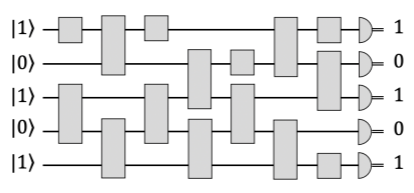
\includegraphics[width=0.5\linewidth]{Images/quantum-circ.png}
    \caption{Generic form of a Quantum Circuit}
    \label{fig:quantum-circ}
\end{figure}
The input gate is on the left, as computational basis states. Data flows from left to right as a series of unitary gates. Then measurement gates occur at the end, which yields the output of the computation.
\begin{figure}[ht]
    \centering
    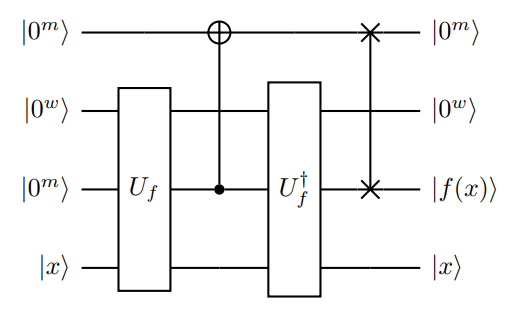
\includegraphics[width=0.8\textwidth]{Images/uncomputation.png}
    \caption{Uncomputation of a classical gate}
    \label{fig:uncomp}
\end{figure}
Again, we can take various cost measures of quantum circuits, such as the number of gates, the depth, or the width. Let's focus on the number of gates. As with classical circuits, we need a notion of what an elementary gate is. For now let's consider the elementary gates to be the set of all 1-qubit and 2-qubit gates. We'll consider simpler gates later on.
    
Consider the factoring problem again. Peter Shor's famous factoring algorithm can be expressed as a quantum circuit for factoring that consists of $O(n^2 \log n)$ gates - a polynomial number of gates! An efficient implementation of this algorithm would break several cryptosystems, whose security is based in the presumed computational hardness of factoring.



\section{Fault tolerant Computation}
We assumed that quantum operations can be perfectly performed and all errors come from either approximation errors at the mathematical level,
or Monte Carlo errors in the readout process due to its probabilistic nature of the measurement process.
Note that because of technical difficult quantum gates, and measurements involve significant errors on near-term quantum devices.
\begin{theorem}
    \textbf{Threshold theorem:} If the noise in individual quantum gates is below a certain constant threshold (around $10^{-4}$ or above) it is possible to perform an arbitrarily large computation with any desired precision. This requires quantum error correction protocols.
\end{theorem}


